\documentclass[11pt,letterpaper]{article}
\usepackage[margin=0.85in]{geometry}
\usepackage{amsmath,amssymb,booktabs,array,longtable,graphicx}
\usepackage{xcolor,enumitem,fancyhdr,float,hyperref}
\hypersetup{colorlinks=true,linkcolor=blue!45!black,urlcolor=blue!45!black,
 citecolor=blue!45!black,pdftitle={Ember: the long life of a 0.1 solar-mass star},
 pdfauthor={Ember project, prepared for Gregory Laughlin}}
\graphicspath{{./}}
\setlength{\parindent}{0pt}\setlength{\parskip}{6pt}
\setlength{\emergencystretch}{2em}\setlist{nosep,leftmargin=*}
\pagestyle{fancy}\fancyhf{}
\fancyhead[L]{\small Ember\quad Working paper}
\fancyhead[R]{\small 27 September 2026}
\fancyfoot[C]{\small\thepage}\setlength{\headheight}{14pt}
\newcommand{\Ms}{M_\odot}\newcommand{\Rs}{R_\odot}\newcommand{\Ls}{L_\odot}
\newcommand{\Tyr}{\mathrm{Tyr}}
\newcommand{\Teff}{T_{\rm eff}}
\begin{document}
\begin{center}
{\Large\bfseries Ember: the long life of a $0.1\Ms$ star}\\[8pt]
{\small Working paper, 27 September 2026}
\end{center}

% Generated from the preserved continuous trajectory.
\newcommand{\continuousAge}{3.615}
\newcommand{\continuousTemperature}{3497}
\newcommand{\continuousHydrogen}{0.2777}
\newcommand{\continuousRadius}{0.142}
\newcommand{\continuousLuminosity}{0.002715}
\newcommand{\continuousCoreTemperature}{10.91}
\newcommand{\continuousCPUHours}{17.37}
\newcommand{\continuousAccepted}{9593}
\newcommand{\pmsTemperature}{2763}
\newcommand{\pmsRadius}{0.1265}
\newcommand{\pmsLuminosity}{0.0008401}
\newcommand{\pmsNuclearPercent}{99.09}
\newcommand{\pmsCoreTemperature}{4.622}
\newcommand{\pmsHeThree}{0.0002376}
\newcommand{\pmsRadiusExcessPercent}{1.186}
\newcommand{\pmsAccepted}{1000}
\newcommand{\continuousRejected}{956}
\newcommand{\continuousRadiativePercent}{72.32}
\newcommand{\continuousNuclearPercent}{99.71}

\section*{Summary}
Ember is a one-dimensional stellar-evolution code written to follow a
$0.1\Ms$ star from contraction, through hydrogen burning lasting several
trillion years, to a cooling helium white dwarf and its conditional fate if
nucleons decay.

A continuous calculation, started on the Hayashi track and run with one
program from deuterium burning onward, has passed $3.02\Tyr$ at 3121 K,
with the star still fully mixed and hydrogen at $X=0.2734$. This run uses a
bounded fixed-metal atmosphere. A second calculation selects the measured
metal- and hydrogen-dependent atmosphere families from the same Hayashi
starting prescription. Neither has yet reached the late burning shell.

A comparison calculation, started from a static hydrogen-burning
model on its own clock, includes gravitational settling of helium and
metals and reaches $4.002\Tyr$. Whole-star convection ends near
$3.55\Tyr$, central hydrogen falls below one part in a thousand near
$3.65\Tyr$, and luminosity and surface temperature pass shallow maxima
($0.006513\Ls$; 4754 K) before the model turns down at 4612 K, still
97\% powered by hydrogen burning. A companion calculation without settling
is about twice as luminous as the 1997 model of Laughlin, Bodenheimer and
Adams at the same mass and reaches each burning stage in about 60\% of the
time; MESA runs with grey atmospheres show the same sequence of events.

When the outer boundary of the settling model is switched to a published
pure-hydrogen white-dwarf atmosphere, a helium-3 shell flash develops. It
appears on every mass grid and mixing treatment tried, but every computed
history descends from one post-switch state, the shell was fading before
the switch, and no other calculation shows it. Its peak, its duration and
whether it occurs with the original boundary are not established; the
continuations through it are provisional, and the control with the
original atmosphere is pending.

The continuous settling calculation still needs atmosphere coverage through
cooling below 4600 K, coupled grain formation, hydrogen-free atmospheres and
a cold helium equation of state. Grey-atmosphere comparisons already reach
lower temperatures. The paper ends with a conditional timeline to the loss
of the remnant.

\section{The question and the calculations}
A star of $0.1\Ms$ burns hydrogen for several trillion years. Laughlin,
Bodenheimer and Adams \cite{lba97} (LBA97) followed its evolution into
white-dwarf cooling with a grey atmosphere and the opacities and reaction
rates of the 1990s. The aim of Ember is to follow such
a star from formation through hydrogen exhaustion, the transition to a helium
white dwarf, cooling through 1000, 500 and 100 K, and the conditional stages
that follow: encounters, accretion, dark-matter heating, and disappearance if
nucleons decay. The remit is to use the simplest model that resolves each
question and to keep numerical uncertainty below about a tenth of the
physical variation that matters.

The paper reports five calculations. Their clocks differ and they have not
been joined into one track.
\begin{itemize}
\item The \textbf{continuous calculation} starts from a Hayashi-track model
and runs deuterium, proton--proton and CN burning, plasma neutrino losses and
convective mixing in one program. With hot microscopic transport and
composition-dependent atmospheres it reaches $\continuousAge\Tyr$.
Age is measured from the contracting starting model (Section~\ref{sec:contraction}).
\item \textbf{Track S} (settling) starts from a static hydrogen-burning model
at age zero and follows hydrogen, helium-3, carbon, nitrogen and a moving
metal group with microscopic diffusion and settling. It reaches
$4.002\Tyr$ and supplies the initial state of the flash comparisons.
\item \textbf{Track F} (fixed metals) uses the same network and diffusion
with the metal abundance held fixed; it reaches $3.704\Tyr$.
\item \textbf{Track P} (proton--proton only) omits carbon--nitrogen burning
and microscopic diffusion; it reaches $3.890\Tyr$ and is the basis of the
LBA97 comparison.
\item The \textbf{flash continuations} F1 and F2 start from Track S after
its outer boundary is replaced by a pure-hydrogen white-dwarf table. They are
provisional (Section~\ref{sec:flash}).
\end{itemize}

Sections~\ref{sec:model}--\ref{sec:hydrogen} give the model, the
contraction results and the hydrogen-burning results. Section~\ref{sec:flash}
separates what is established about the helium-3 flash from what is not.
Section~\ref{sec:comparisons} compares with LBA97, with MESA and with
observed stars. Section~\ref{sec:limits} lists the missing physics that can
change the interpretation, Section~\ref{sec:lifetime} gives the conditional
lifetime timeline, and Section~\ref{sec:computing} records cost and
reproducibility. The appendix holds reusable implementation detail.
Every number in the text is a calculated value unless labelled as a
literature value or a conditional estimate. Table~\ref{tab:status}
summarizes the status of each calculation.

\begin{table}[H]\centering\small
\caption{Status of the calculations reported here.}\label{tab:status}
\begin{tabular}{@{}>{\raggedright\arraybackslash}p{0.19\textwidth}>{\raggedright\arraybackslash}p{0.18\textwidth}>{\raggedright\arraybackslash}p{0.26\textwidth}>{\raggedright\arraybackslash}p{0.28\textwidth}@{}}\toprule
Calculation & Clock & Last computed state & Status \\\midrule
Continuous calculation & from Hayashi model & $\continuousAge\Tyr$, \continuousTemperature\ K, surface $X=\continuousHydrogen$ & radiative core, convective envelope \\
Fixed-metal atmosphere comparison & from Hayashi model & $3.078\Tyr$, 3130 K & complete comparison; fully convective \\
Track S & static H-burning model & $4.002\Tyr$, 4612 K & complete to atmosphere limit \\
Track F & static H-burning model & $3.704\Tyr$, 3702 K & complete (comparison) \\
Track P & static H-burning model & $3.890\Tyr$, 5546 K & complete (comparison) \\
Flash continuations F1, F2 & from post-switch model & 5.744 Myr; 42.48 Myr & provisional; no continuous flash \\
Continuous settling calculation & from Hayashi model & below 4600 K & further cooling needs opacity and atmosphere coverage \\\bottomrule
\end{tabular}
\end{table}

\section{The model}\label{sec:model}
All calculations hold the baryonic mass fixed at $0.1\Ms$ and omit rotation,
magnetism, mass loss, accretion and external heating. The initial hydrogen
mass fraction is $X=0.7$ and the metal fraction $Z=0.02$, with the relative
metal abundances of the Grevesse--Sauval (GS98) mixture and the remainder in
$^4$He. Tracks S, F and P start with no $^3$He; the continuous calculation
starts with initial deuterium. Table~\ref{tab:ingredients} distinguishes
the physical assumptions of the comparison tracks from those selected for
the continuous calculation.

{\small\renewcommand{\arraystretch}{1.12}
\begin{longtable}{@{}>{\raggedright\arraybackslash}p{0.13\textwidth}>{\raggedright\arraybackslash}p{0.44\textwidth}>{\raggedright\arraybackslash}p{0.37\textwidth}@{}}
\caption{Physical ingredients by calculation.}\label{tab:ingredients}\\
\toprule Component & Tracks S, F, P and flash continuations & Continuous calculation \\\midrule\endfirsthead
\toprule Component & Tracks S, F, P and flash continuations & Continuous calculation \\\midrule\endhead
Starting model & Static, fully convective hydrogen-burning model at age zero:
$R=0.1259\Rs$, $\Teff=2766$ K, $L=0.0008362\Ls$, central density
381.7 g cm$^{-3}$. & Fully convective Hayashi-track model: $\Teff=2864$ K,
$R=1.594\Rs$, central temperature 0.5398 MK, with initial deuterium. \\[4pt]
Nuclear reactions & Reduced ppI/ppII network with $^3$He out of equilibrium,
Solar Fusion II rates \cite{adelberger11} and finite-degeneracy Salpeter--Van
Horn screening. Tracks F and S add a time-dependent CN cycle ($^{12}$C,
$^{13}$C, $^{14}$N) with the $^{14}$N capture rate of Solar Fusion III
\cite{acharya25}; in Track S nuclear captures change the metal mass. Track P
has no CN burning. Pep, hep, ppIII and the oxygen branches are absent in all.
& Initial deuterium, pp and closed CN burning with Solar Fusion III rates
for both networks and the same screening prescription.
Pep, hep, ppIII and oxygen branches absent. \\[4pt]
Heat transport & Mixing-length convection with the Ledoux criterion;
radiative opacity plus electron conduction from Ioffe/Cassisi mixtures;
plasma-neutrino losses \cite{hrw94}. Other thermal-neutrino processes are
omitted. & Ledoux mixing-length convection, radiation, plasma-neutrino
losses and conductive heat transport. In hot layers the screened kinetic
calculation supplies the conductive coefficient; it joins the cool-envelope
Ioffe/Cassisi coefficient smoothly between 2 and 3 MK. \\[4pt]
Composition transport & Track P: instantaneous mixing within each convective
region, slow mixing in marginally stable layers, no microscopic diffusion.
Track F: microscopic diffusion of H, $^3$He, C and N with the metal
inventory fixed; chemical forces from the equation-of-state free energy;
electron collisions averaged over the finite-temperature Fermi distribution.
Track S: as F, with all heavy elements moving as one group with distinct
charges, and the equation of state and opacity depending on the total metal
abundance. Flash continuations: finite mixing $D=v\ell/3$ in hot convective
regions; semiconvective and thermohaline coefficients set to zero.
& Instantaneous whole-star mixing while the star is fully convective, with
the heat carried by changing composition included after deuterium
exhaustion. Screened H/He/metal species fluxes act across radiative
boundaries at temperatures of at least 2 MK; the metal law assumes full
ionization. Cooler radiative species transport is unsupported.
The heat law, rather than the species flux, uses the smooth 2--3 MK join. \\[4pt]
Equation of state & FreeEOS 3.0 free-energy tables with numerical electron
integrals, interpolated through a shared Helmholtz potential so that
pressure, energy and composition responses stay consistent. Track P: 72
composition tables. Track F: 152 tables at 38 hydrogen and four $^3$He
fractions. Track S: a variable-metal family from $Z=0$ to 0.08, extended to
0.16 for the metal-enriched core. None describes the cold, dense remnant.
& One interpolated potential with planes at $Z=0$, 0.005, 0.02, 0.04 and
0.16, twelve hydrogen-share coordinates and four $^3$He-share coordinates;
all 512 zones support the required composition derivatives. \\[4pt]
Opacity & AESOPUS 2.1 gas opacity at low temperature (no grains) and Los
Alamos ATOMIC/TOPS opacity at high temperature \cite{colgan16,tops},
including hydrogen-free mixtures above $5.012\times10^5$ K. Composition
continuations in $X$ and $Z$ are given in Appendix~\ref{app:tech}.
& Same tables and continuations. \\[4pt]
Atmosphere & TLUSTY/SYNSPEC plane-parallel LTE atmospheres with
frequency-resolved absorption, scattering and collision-induced absorption,
no condensates, joined to the interior at Rosseland optical depth 100.
Track P: 220 atmospheres over $X=0.1$--0.7, $^3$He 0--0.12, through
5600 K. Track S: additional families down to $Z=10^{-8}$ and $1-X=10^{-5}$,
4600--6000 K, $\log g$ to 5.95, with a local continuation to 6.1. Flash
continuations: the pure-hydrogen white-dwarf table distributed with MESA
\cite{rohrmann11,mesa_atm}, joined at optical depth 25.12 and extrapolated
below $\log g=5.5$. & A composition-dependent family at $X\geq0.65$,
$^3$He $\leq0.0075$, fixed $Z=0.02$, joined at optical depth 100. The
continuous metal-dependent selection joins measured families through
nearly pure hydrogen, including trace helium, at the same optical depth.
The 4600 K gravity row and its high-gravity corner have solved source
columns; intermediate knots interpolate the sources. Trace helium remains
approximated. Coverage ends at 4600 K and $\log g=6.1$. \\[4pt]
Mesh and time integration & 512 mass points, fixed for Tracks S, F and P;
flash grids refined locally to 578--2115 points. Structure, burning and
mixing are solved together implicitly. Every accepted step is compared with
two half steps; species inventories, inert-metal mass, nuclear rest-mass
release and the first law are checked independently. Saved models restart
exactly. & 512 zones; the same step-doubling check; independent isotope,
mass-defect and first-law audits on every interval; exact restart replay.
Radiative-core evolution and restart are registered tests. \\
\bottomrule
\end{longtable}}

For Tracks S, F and P the relative time-error tolerances are 0.0003 for radius, density and
temperature, 0.003 for local $^3$He and 0.001 for the other species; the
abundance solver converges to $10^{-10}$. Tightening the structure and
$^3$He tolerances threefold over a matched 5 Gyr interval changes luminosity
by 0.002872\% and surface temperature by 0.01705 K, while loosening the
structure tolerance to 0.001 over 2 Gyr changes luminosity by 1.078\% and
temperature by 3.114 K; the tracks therefore keep the original settings.
The continuous calculation uses a structure tolerance of $10^{-4}$ and an
energy tolerance of 0.005. Local composition solves converge to $10^{-15}$
in a single instantaneously mixed region and $10^{-12}$ in a stratified
star; the separate global abundance-balance tolerance remains $10^{-14}$.

Throughout the paper a \emph{paired comparison} means two calculations
started from the same model, differing in one setting, and compared at the
same age. Such comparisons measure sensitivity to that setting over the
stated interval; they are not error bounds for a complete lifetime, and the
text says so wherever the distinction matters.

Replacing the Solar Fusion II rates by Solar Fusion III with everything else
fixed raises the initial luminosity by 0.7454\% and the radius by 0.2164\%.
FreeEOS omits potassium (mass fraction $4.56\times10^{-6}$). The interior
equation of state, atmosphere chemistry, opacity and conduction come from
different sources; their mutual consistency is checked at sampled states
(Appendix~\ref{app:tech}) rather than guaranteed.

\section{Contraction and the continuous calculation}\label{sec:contraction}
The contraction calculation starts from a fully convective model at
$\Teff=2864$ K and $R=1.594\Rs$. Initial deuterium burns first and is
exhausted; proton--proton burning then rises to supply the surface
luminosity (Figure~\ref{fig:pms}). At 1 Gyr the model has $\Teff=2765$ K,
$R=0.1264\Rs$, $L=8.416\times10^{-4}\Ls$, central temperature 4.623 MK and
$\log g=5.234$, with nuclear burning supplying 99.17\% of the light. The
abundances are still uniform, $X=0.6998$ and $X_3=2.402\times10^{-4}$.
The sequence to 1 Gyr contains 1019 accepted intervals and no rejected ones,
and every interval passes the step-doubling, isotope, mass-defect and
first-law checks. Continued with the same settings, the star reaches 4 Gyr
with sustained hydrogen burning; allowing steps up to 1 Gyr on the quiet
main sequence changes the endpoint temperature by $6.936\times10^{-5}$ K.

\begin{figure}[H]\centering
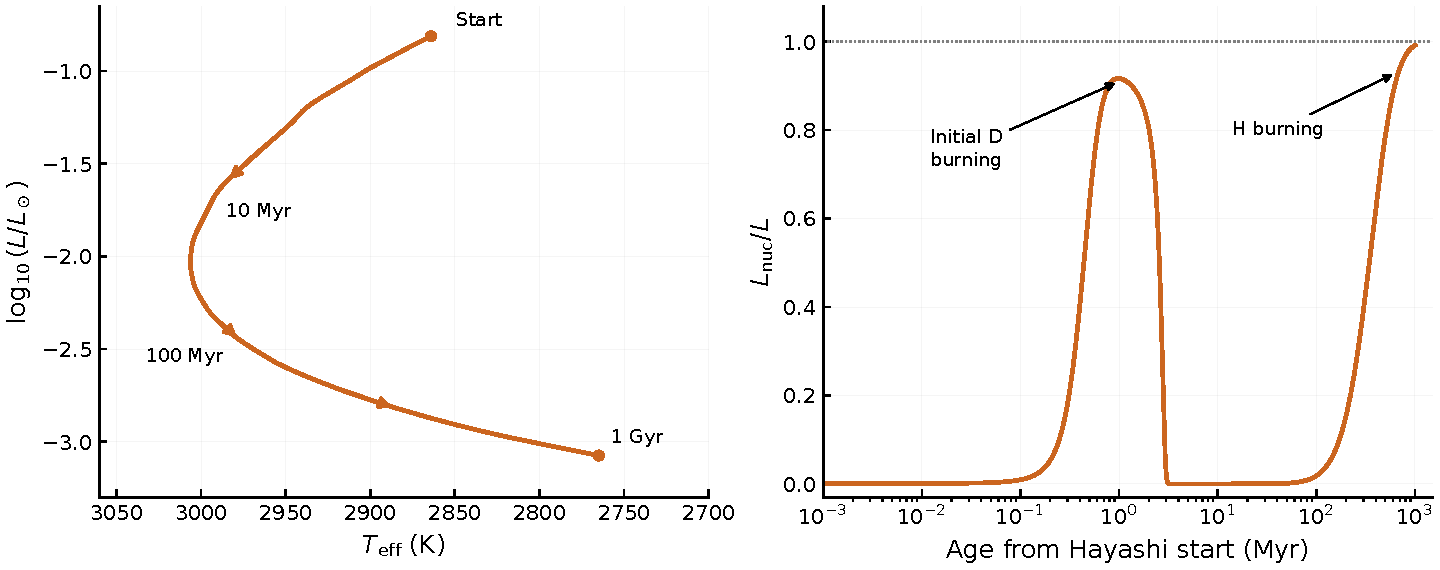
\includegraphics[width=0.92\textwidth]{pms_main_sequence.pdf}
\caption{Contraction of the $0.1\Ms$ model into the main sequence,
computed with the continuous driver. Left: the HR track, arrows showing
increasing age. Right: the fraction of the surface luminosity supplied by
nuclear burning; the early maximum is deuterium burning. Age is measured
from the contracting starting model. The plotted sequence ends at 1 Gyr;
the same calculation continues to 4 Gyr and, with the composition-dependent
atmosphere, to $2.102\Tyr$ (text). It is not joined to Tracks S, F and P.}
\label{fig:pms}
\end{figure}

During deuterium burning the convective travel time is 0.9535--1.415 yr
against local burning times of at least 1949 yr, and the heat carried by
composition redistribution is at most 0.003463\% of the local luminosity;
including ten times that heat produces no resolved change. After deuterium
exhaustion, generous estimates of neutral and Coulomb mobilities give a
microscopic-to-convective diffusion ratio below $6.581\times10^{-9}$, and
ten times the estimated kinetic heat changes the 1 Gyr endpoint by less than
$10^{-3}$ K. These estimates justify whole-star instantaneous mixing while
the star is fully convective; they are not a transport law for partially
ionized gas, and the approximation ends when a radiative region forms.

\paragraph{Comparison with observed stars.}
Table~\ref{tab:observed} compares the continuous model at 1 Gyr with
three measured objects \cite{davis24,agol21,ribas17}. The closest comparison
is the eclipsing companion EBLM J2114$-$39 B, whose mass agrees with
$0.1\Ms$ and whose radius is 1.1\% smaller than Ember's, within its
uncertainty; its metallicity, $[\mathrm{Fe/H}]=-0.001\pm0.032$, matches the
adopted composition. TRAPPIST-1 and Proxima bracket Ember in radius,
temperature and luminosity, but their masses rest on a mass--luminosity
relation and on stellar models respectively. Ten billion years of hydrogen
burning changes Ember's luminosity by less than 0.4\% and its temperature
by less than 2 K, so main-sequence age does not affect the comparison.
The agreement supports the starting structure without establishing
percent-level accuracy or selecting among atmosphere and interior choices.

\begin{table}[H]\centering\small
\caption{Continuous model at 1 Gyr and observed low-mass stars.}\label{tab:observed}
\begin{tabular}{@{}lrrrr@{}}\toprule
Star & Mass ($\Ms$) & Radius ($\Rs$) & $\Teff$ (K) & Luminosity ($\Ls$) \\\midrule
Ember, 1 Gyr & 0.1 & 0.1264 & 2765 & 0.0008416 \\
EBLM J2114$-$39 B & $0.0993\pm0.0033$ & $0.1250\pm0.0016$ & --- & --- \\
TRAPPIST-1 & $0.0898\pm0.0023$ & $0.1192\pm0.0013$ & $2566\pm26$ & $0.000553\pm0.000019$ \\
Proxima & $0.120\pm0.003$ & $0.146\pm0.007$ & $2980\pm80$ & $0.00151\pm0.00008$ \\\bottomrule
\end{tabular}
\end{table}

\paragraph{Continuous hydrogen burning.}
The same program follows contraction, deuterium burning and the main
sequence using composition-dependent atmosphere tables at fixed $Z=0.02$.
A completed calculation reaches $2.102\Tyr$ in 5931 accepted intervals,
66.16 CPU minutes and 35.41 minutes of elapsed time. At that age the star
is still fully mixed, with $X=0.4170$, $\Teff=3020$ K,
$R=0.1485\Rs$, $L=0.001653\Ls$ and central temperature 5.921 MK.
Every accepted interval passes the isotope and energy audits. The
fixed-metal allowance of $10^{-8}$ ultimately rejects 28 trial intervals;
the final, repeatedly halved trial fails the separate energy audit. This
limit belongs to the chosen atmosphere approximation, rather than to an
instability in the accepted stellar structures.

With hot screened transport selected and a fixed-metal allowance of
$2\times10^{-5}$, the continuous model has passed $3.02\Tyr$ with no
rejected intervals. It remains fully convective. A calculation that includes
the restored hydrogen- and metal-dependent atmospheres starts from the same
Hayashi prescription; its initial contraction and relocated restart pass the
same audits. The material selection covers the saved settling structures
through $X=0.9995$ and $Z=10^{-6}$; the trace-helium and white-dwarf
extensions are still needed. Neither continuous calculation has yet reached
the loss of full convection. Tracks S, F and P therefore provide the
late hydrogen-burning comparisons in Section~\ref{sec:hydrogen}.

\section{Hydrogen burning through four trillion years}\label{sec:hydrogen}

\subsection{The three long-term tracks}
Tracks S, F and P start from the same kind of static hydrogen-burning model
and differ in nuclear network and composition transport
(Table~\ref{tab:ingredients}). Figure~\ref{fig:hr} shows all three in the
HR diagram with the LBA97 track; Figure~\ref{fig:composition} shows the
composition and convection histories. Table~\ref{tab:milestones} lists the
computed milestones by track.

\begin{figure}[H]\centering
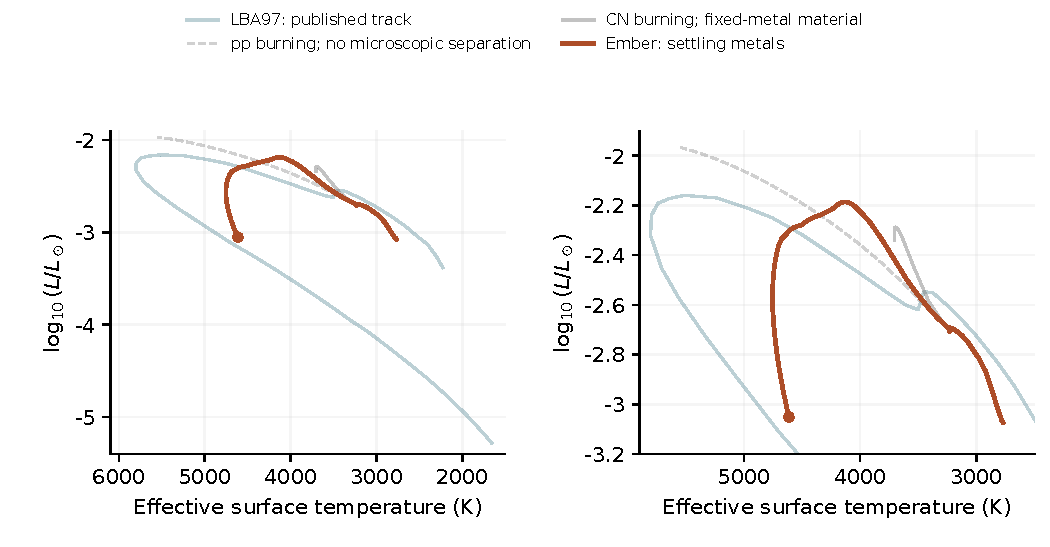
\includegraphics[width=\textwidth]{lba97_hr.pdf}
\caption{HR diagrams of Track S (orange, through $4.002\Tyr$), Track F
(solid gray, through $3.704\Tyr$), Track P (dashed gray, through
$3.890\Tyr$) and the published LBA97 track (pale blue, read from its
Figure~1 without age rescaling). Left: full range; right: the
hydrogen-burning portion. Track P differs from S in both nuclear and
transport physics, so the separation between them is not the effect of
settling alone. The small luminosity dip near 3230 K accompanies the
formation of an interior radiative layer.}
\label{fig:hr}
\end{figure}

\begin{table}[H]\centering\small
\caption{Computed milestones. Ages in Tyr on the long-term clock; ``---''
means not reached or not recorded for that track.}\label{tab:milestones}
\begin{tabular}{@{}lrrr@{}}\toprule
Event & Track S & Track F & Track P \\\midrule
Maximum central $^3$He (mass fraction) & --- & --- & 0.7103 (0.1003) \\
Loss of full convection (central $X$) & $\simeq3.55$ & 3.549 (0.1744) & 3.546 (0.1751) \\
Centre becomes radiative & 3.551 & 3.551 & --- \\
Central $X=10^{-3}$ & 3.650 & 3.661 & --- \\
Central $X=10^{-4}$, $10^{-5}$ & 3.660, 3.767 & --- & --- \\
Luminosity maximum ($\Ls$; $\Teff$) & 3.673 (0.006513; 4128 K) & 3.677 (0.005163; 3695 K) & --- \\
Surface-temperature maximum & 3.838 (4754 K) & 3.689 (3705 K) & --- \\
Last computed model & 4.002 & 3.704 & 3.890 \\
\quad $\Teff$ (K) & 4612 & 3702 & 5546 \\
\quad central $X$ & $3.528\times10^{-8}$ & $1.309\times10^{-4}$ & $8.157\times10^{-4}$ \\
\quad surface $X$ & 0.9982 & 0.8905 & 0.1730 \\
\quad convective mass fraction & 0.01553 & --- & 0.02565 \\
\quad nuclear share of luminosity & 97.28\% & --- & --- \\\bottomrule
\end{tabular}
\end{table}

At its endpoint Track S has $R=0.04667\Rs$, $L=0.0008881\Ls$, central
temperature 6.443 MK, central density $3.982\times10^4$ g cm$^{-3}$,
central metal fraction 0.1312, surface metal fraction below $10^{-40}$,
and $0.003797\Ms$ of hydrogen remaining. Surface temperature has declined
by 141.5 K over the 164.3 Gyr since its maximum, but hydrogen burning still
supplies 97.28\% of the light; the model has turned toward cooling but is
not yet on a passive cooling sequence.

\begin{figure}[H]\centering
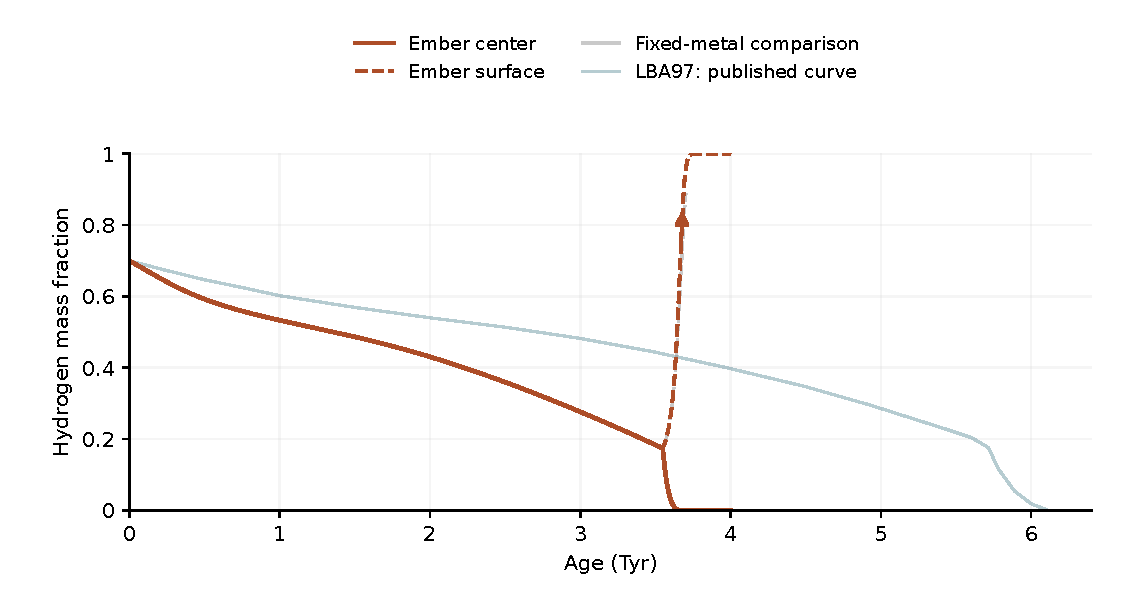
\includegraphics[width=0.7\textwidth]{hydrogen_evolution.pdf}\\[2pt]
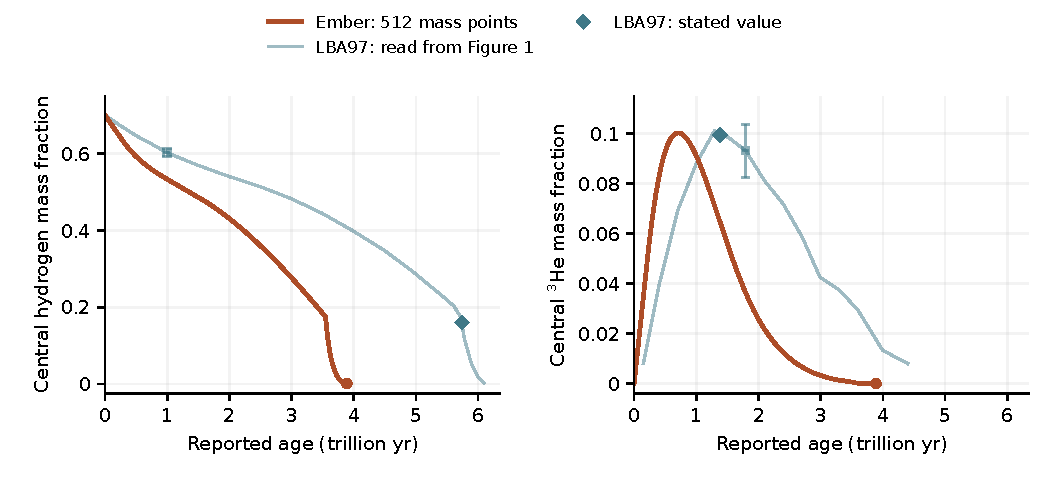
\includegraphics[width=0.7\textwidth]{lba97_composition.pdf}\\[2pt]
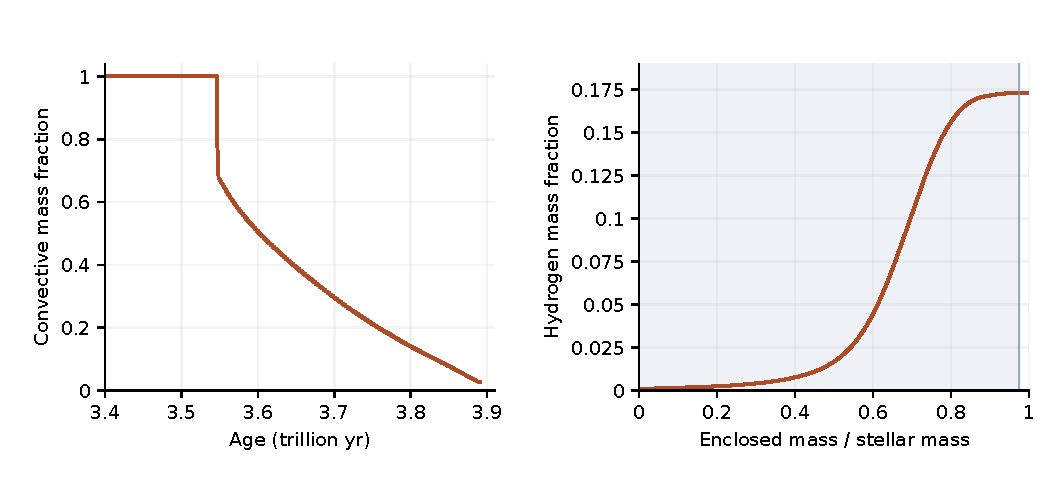
\includegraphics[width=0.7\textwidth]{convection_current.pdf}
\caption{Composition and convection histories. Upper: central (solid) and surface (dashed)
hydrogen for Track S (orange) and Track F (gray), with the LBA97 curve in
pale blue; the arrow follows increasing age along the Track S surface curve.
Lower: hydrogen and $^3$He in Track P (orange) against the LBA97 inset (pale
curves, read from the printed figure; diamonds mark LBA97's stated $^3$He
maximum and the hydrogen abundance at radiative-core formation). Crosses
show the reading precision of four image pixels, about $0.05\Tyr$ and 0.01
in mass fraction. Ages are shown as reported, without rescaling. Lower:
Track P's convective mass fraction, declining from unity near $3.546\Tyr$
to 0.02565 at $3.890\Tyr$, and its hydrogen profile at $3.890\Tyr$; the
shaded core carries heat by radiation and conduction.}
\label{fig:composition}
\end{figure}

\subsection{The end of full convection and the conductive core}
Track P first departs from full convection near $3.546\Tyr$ at central
$X=0.1751$: a radiative layer separates the convective centre from the
envelope. By $3.560\Tyr$ the convective mass fraction has fallen to 0.6277
and central hydrogen to 0.1518 while the surface remains at 0.1747, so the
star is no longer mixed as a whole. In Track F the same transition occurs
near $3.549\Tyr$ (3230 K, central $X=0.1744$) and the central convective
region disappears near $3.551\Tyr$. At that transition carbon-12 depletion
is 0.02652, with 0.02524 accumulated as carbon-13 and only 0.001275
converted to nitrogen: the two proton captures cannot be treated as an
instantaneous conversion of carbon to nitrogen during this phase.

At $3.890\Tyr$ Track P has a core containing 97.43\% of the mass that
carries heat by radiation and conduction beneath a convective envelope.
Central hydrogen is $8.157\times10^{-4}$ while the envelope remains near
0.1730. Conduction supplies 91.29\% of the central heat flux; in Track S at
$3.688\Tyr$ electron conduction supplies 99.79\%, with conductive and
radiative coefficients of $1.058\times10^{14}$ and $2.221\times10^{11}$
erg cm$^{-1}$ s$^{-1}$ K$^{-1}$ and a central degeneracy parameter of
15.39. The composition gradient also suppresses convection.
``Fully convective'' describes where convection occurs, not the fraction of
the luminosity it carries; radiation, conduction and convection share the
heat flow continuously, and the mixing-length treatment makes the convective
share go to zero at a stability boundary. Chemical mixing uses the stronger
approximation that each connected convective region becomes uniform quickly.

During the transition in Track F, a mainly radiative layer at enclosed mass
fractions 0.1770--0.2391 separates a convective core from the envelope.
Conduction supplies 4.4--4.8\% of its diffusive heat flow, yet removing
conductivity on that fixed structure would make the layer unstable under the
Ledoux criterion: conduction matters for the convection threshold even where
radiation carries most of the heat.

\subsection{What settling and diffusion change}
At their respective luminosity maxima, Track S is 26.13\% more luminous and
10.03\% smaller than Track F (Table~\ref{tab:lmax}), with nearly equal
central temperatures. Figure~\ref{fig:peak} compares the structures. Near
$3.673\Tyr$ the layer enclosing 80\% of the mass is hotter and denser with
settling, 8.260 rather than 7.402 MK and 489.6 rather than 245.0 g
cm$^{-3}$, and poorer in hydrogen, $X=0.1726$ rather than 0.2712; integrating
the reaction rates gives 27.25\% more nuclear power. Track S has consumed
0.4987\% more hydrogen than Track F at this point (80.83\% against 80.43\% of
the initial inventory). CN reactions contribute 1.286\% of its nuclear
power. The coupled tracks do not isolate the separate contributions of
atmospheric opacity, interior material properties and diffusion.

\begin{table}[H]\centering\small
\caption{Structure at the luminosity maximum.}\label{tab:lmax}
\begin{tabular}{@{}lrr@{}}\toprule
 & Track F & Track S \\\midrule
Age (Tyr) & 3.677 & 3.673 \\
Luminosity ($\Ls$) & 0.005163 & 0.006513 \\
Effective temperature (K) & 3695 & 4128 \\
Radius ($\Rs$) & 0.1753 & 0.1578 \\
Central temperature (MK) & 11.90 & 11.97 \\
Remaining hydrogen ($\Ms$) & $\simeq0.01370$ & 0.01342 \\
Convective mass fraction & 0.05536 & 0.03339 \\\bottomrule
\end{tabular}
\end{table}

\begin{figure}[H]\centering
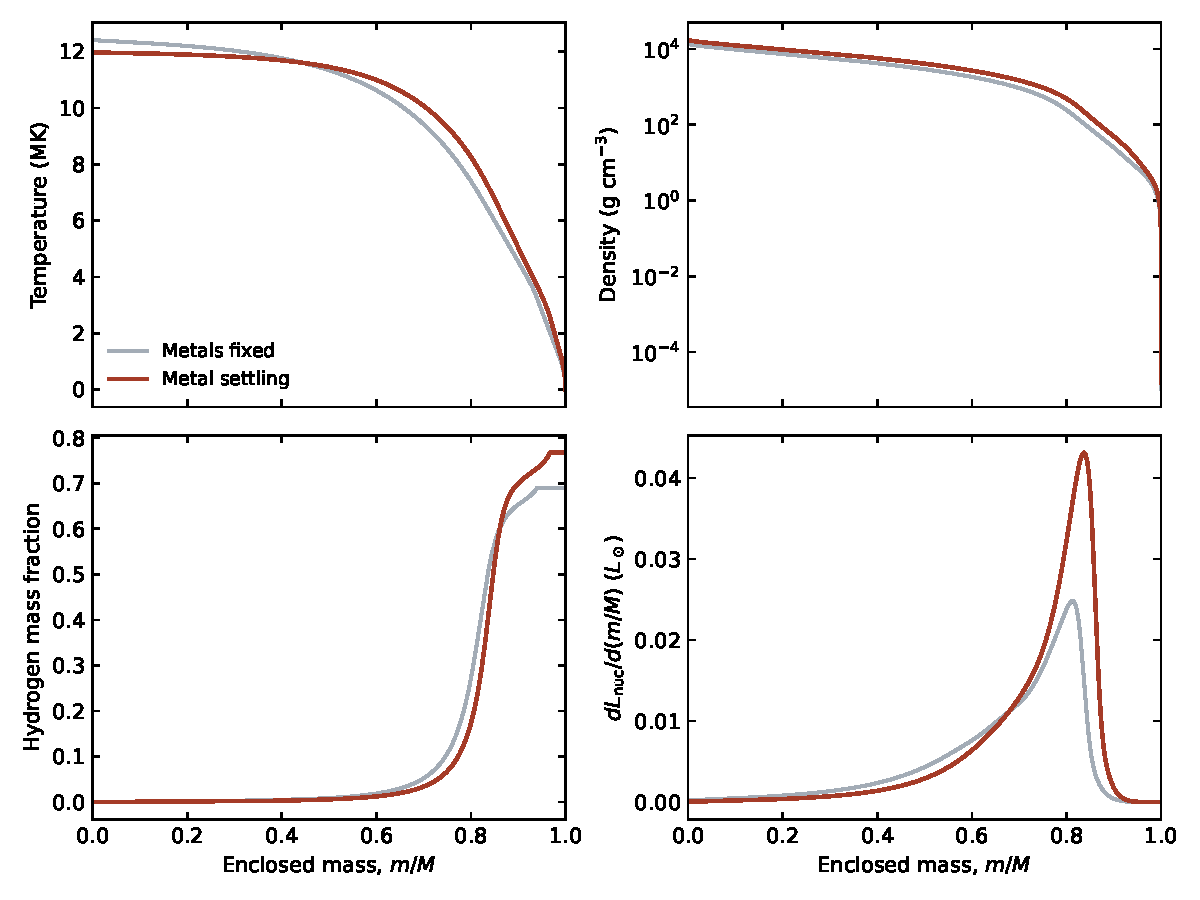
\includegraphics[width=0.93\textwidth]{metal_peak_structure.pdf}
\caption{Temperature, density, hydrogen abundance and nuclear power per unit
fractional mass at the Track S luminosity maximum, compared with a Track F
structure of nearly the same age (0.1837 Gyr later; not the Track F
maximum). The strongest burning occurs outside the depleted centre. The
curves compare actual structures; exchanging their profiles would not
produce equilibrium models.}
\label{fig:peak}
\end{figure}

\paragraph{Diffusion alone.}
A paired comparison from the same $3.560\Tyr$ Track F structure, evolved
50 Gyr with and without microscopic drift, gives central $X=0.02300$ with
drift and 0.06864 without, surface $X=0.2907$ and 0.1847, and effective
temperatures of 3404 and 3302 K. Total remaining hydrogen differs by only
0.2767\%, but the diffusive calculation burns 4.241\% more hydrogen during
the interval and ends 20.10\% more luminous. Over this interval diffusion
mainly redistributes fuel and changes the structure that burns it. Ember's
drift speeds at 14 weakly degenerate interfaces are 0.8163--0.9258 of the
classical Thoul--Bahcall--Loeb values \cite{thoul94}; the degenerate core
needs the actual gravity and electron thermodynamics \cite{paxton18}.

For a nearly homogeneous radiative centre, a drift speed of order
$Dm_pg/(kT)$ gives a separation time
\begin{equation}
 t_{\rm sep}\sim\frac{kT}{4\pi G\rho m_pD},
\end{equation}
of order 100 Gyr at $T\sim9$ MK, $\rho\sim300$ g cm$^{-3}$ and
$D\sim0.7$ cm$^2$ s$^{-1}$. Separation therefore competes with the final
core-burning phase while having little effect during the much longer fully
convective phase. The residual-fuel scale
\begin{equation}
 t_{\rm fuel}\sim10^{12}\,{\rm yr}\left(\frac{\Delta M_{\rm H}}{10^{-3}\Ms}\right)
 \left(\frac{L}{10^{-4}\Ls}\right)^{-1}
\end{equation}
shows why a central hydrogen threshold alone does not fix the duration of
shell burning: the energy is available only if hydrogen reaches layers hot
enough to burn, and diffusion controls that supply. LBA97 held the envelope
composition nearly fixed after the radiative core formed and included no
microscopic diffusion; its final whole-star hydrogen fraction is slightly
above 0.01 while its envelope retains $X=0.155$. The tracks here differ from
it in exactly the process that decides how much of that envelope hydrogen
ever burns.

\paragraph{Settling of metals.}
In Track S the surface-connected convective envelope shrinks from 4.716\%
of the mass at $3.664\Tyr$ to 2.013\% at $3.727\Tyr$ while its hydrogen
fraction rises from 0.6804 to 0.9945; helium and metals diffuse downward
through its base and the envelope ends nearly metal-free. A passive
calculation following C, N, O, Na, Mg, Si, Ca and Fe on the Track F
structures from 3.551 to $3.704\Tyr$, with the published collision
coefficients \cite{thoul94}, leaves surface abundances at 0.06213--0.08217
of their initial values with classical heat flow and 0.2491--0.3076 with heat
flow suppressed; the two treatments are alternative approximations, not an
uncertainty band. Halving the time interval changes the surface results by
at most 0.2078\%. Metals accumulate in the conductive core, reaching
$Z=0.1312$ at the Track S endpoint. Accretion could maintain surface metals
against settling \cite{bauer19}; the isolated model has none.

Removing metals from the atmosphere changes the boundary condition
appreciably. At $X=0.85$, 3800 K and $\log g=4.9$, reducing carbon and
nitrogen to 0.1531 and 0.1541 of their initial abundances (the Track F
surface values at $3.697\Tyr$) changes the joining temperature by $+3.314\%$
and the gas pressure by $-4.205\%$; halving all metals changes them by
$-8.606\%$ and $+53.69\%$. Applied as fixed boundary factors to the same
$3.694\Tyr$ structure for 100 Myr, the two changes give
$\Delta\Teff=-30.38$ K and $+142.9$ K, $\Delta L/L=-1.019\%$ and
$+5.041\%$, and $\Delta R/R=+1.142\%$ and $-4.983\%$. These establish an
appreciable surface-temperature response; the actual response in Track S
comes from the transported metal abundance and the metal-dependent
atmosphere families.

\subsection{Measured sensitivities}
Table~\ref{tab:sensitivity} collects the largest effect found for each
class of numerical or table approximation used along Track S. Each entry is
a paired comparison over the stated interval; none is a bound on the full
lifetime. The one entry that is not small is the absolute normalization of
the pure-hydrogen boundary, which is the subject of Section~\ref{sec:flash}.

\begin{table}[H]\centering\small
\caption{Largest measured sensitivities along Track S.}\label{tab:sensitivity}
\begin{tabular}{@{}p{0.36\textwidth}p{0.26\textwidth}p{0.32\textwidth}@{}}\toprule
Approximation tested & Largest table-level discrepancy & Largest stellar response (interval) \\\midrule
Atmosphere interpolation between solved columns (all families, Appendix Table~\ref{tab:atm}) & 2.031\% in $T$, 4.656\% in $P$ at the joining depth & 12.74 K, 0.3110\% in $L$ (30 Gyr) \\
Gravity continuation of the boundary, $\log g=5.95$--6.1 & 0.1878\% in $T$, 2.391\% in $P$ against nine solved atmospheres & 8.697 K, 0.5101\% in $L$ for $\pm0.5\%$/$\pm5\%$ offsets (50 Myr); 60.96 Gyr of track lies inside \\
Temperature continuation of the boundary to 4600 K & solved 4600 K atmosphere agrees within 0.05\% & 17.54 K, 1.026\% in $L$ for $\pm1\%$/$\pm10\%$ offsets (50 Myr) \\
Pure-hydrogen boundary: TLUSTY against the MESA table at 4600 K, $\log g=5.9$ & 2.594\% in $T$, 48.69\% in $P$ & about 241 K in 1 Myr (not converged; Section~\ref{sec:flash}) \\
Molecular opacity continuation below $Z=0.01$ & up to 9.237\% at $Z=0.003$ against withheld sources & 0.002433\% in $L$, 0.009728 K between linear and logarithmic forms (10 Gyr) \\
Radiative opacity $\pm10\%$ in the depleted envelope & --- & 0.6315\% in $L$, 3.216 K (1 Myr) \\
Warm interior opacity $\pm15\%$ (convective layers) & withheld-source differences up to 11.01\%; OPLIB 31.52--35.21\% & below $10^{-10}$ in $L$ and $R$ (1.25 Gyr) \\
Dense-core radiative opacity halved or doubled & --- & no significant change (25 Myr); conduction carries the heat \\
Variable-metal equation of state & 0.7642\% in $c_P$, 1.037\% in $\Gamma_1$ against FreeEOS & below 0.001 K (10 Myr) \\
Core equation of state to $Z=0.16$ & 0.07726\% in material state & 0.0004595 K, 0.0002080\% in $L$ (25 Myr) \\
Time-error tolerances threefold tighter & --- & 0.002872\% in $L$, 0.01705 K (5 Gyr) \\
Structure tolerance loosened to 0.001 & --- & 1.078\% in $L$, 3.114 K (2 Gyr); rejected \\\bottomrule
\end{tabular}
\end{table}

\section{The helium-3 shell flash: a provisional result}\label{sec:flash}

\subsection{Boundary condition and ignition}
Track S ends at $4.002\Tyr$ because its TLUSTY atmosphere families stop
at $\log g=6.1$. To continue, the outer boundary was replaced at that point
by the pure-hydrogen white-dwarf table distributed with MESA
\cite{rohrmann11,mesa_atm}, joined at optical depth 25.12, with the interior
composition and all evolution checks retained. The two prescriptions are not
equivalent: at 4600 K and $\log g=5.9$ the table gives a joining temperature
2.594\% higher and a gas pressure 48.69\% lower than an independently
converged TLUSTY atmosphere, and neither trace helium, the joining depth
(sampled between optical depth 168 and 4775) nor the atmosphere convection
prescription (ML2 with $\alpha=0.6$ and 1.0 change the joining values by
at most 0.04571\% and 0.2736\%) removes the difference. The continuation is
therefore a change of boundary condition, not a refinement.

Figure~\ref{fig:switch} shows the response. The surface temperature first
falls to 4362 K, the radius grows by 36.02\%, and after 0.7546 Gyr, at
$4.003\Tyr$ and 4632 K, the ratio of nuclear to photon luminosity has risen
to 2366: a helium-3 burning shell near $m/M=0.96$ has become convective.
The reaction $^3{\rm He}+{}^3{\rm He}\rightarrow{}^4{\rm He}+2p$ consumes the
accumulated helium-3 and returns hydrogen. Before the switch the shell was
fading, and every flash history computed so far descends from this one
post-switch state.

\begin{figure}[H]\centering
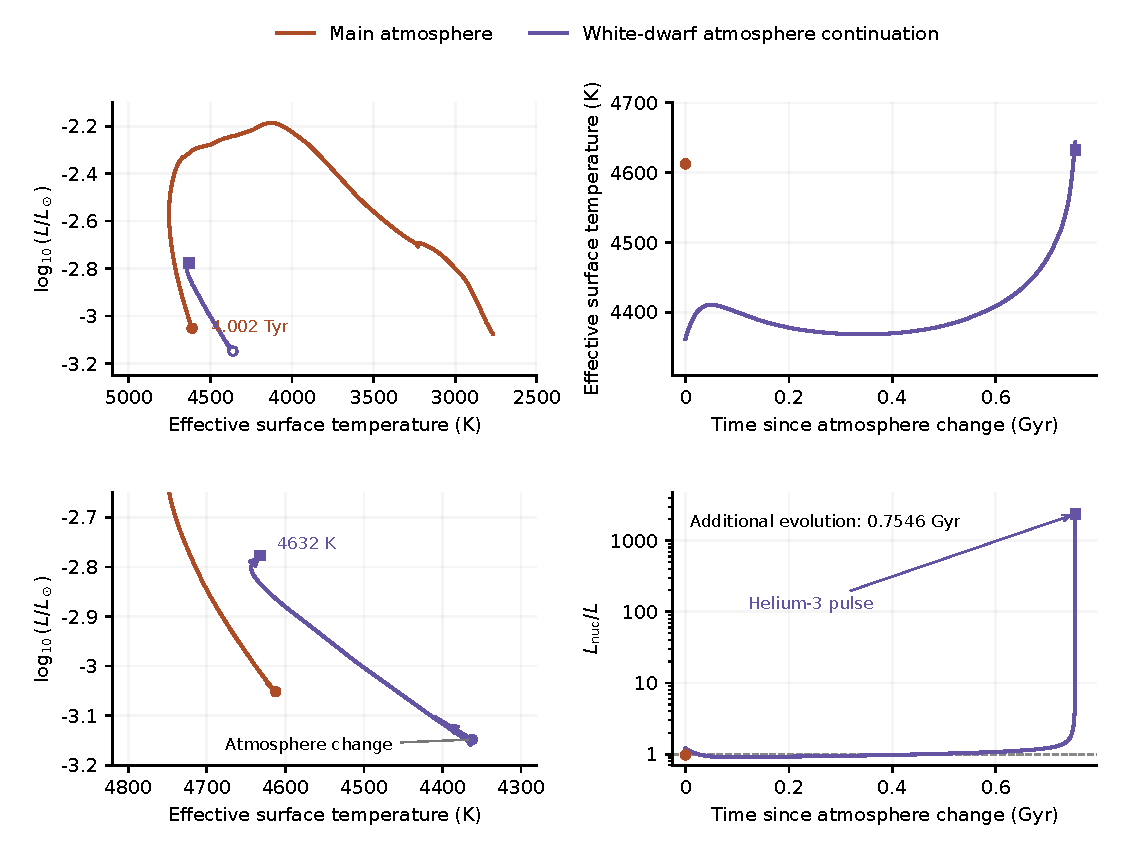
\includegraphics[width=\textwidth]{wd_atmosphere_response.pdf}
\caption{Track S with two atmosphere prescriptions. Orange: the TLUSTY
families through $4.002\Tyr$. Purple: the continuation with the
pure-hydrogen white-dwarf table, which differs from the TLUSTY boundary by
2.6\% in temperature and 49\% in pressure at the joining depth in the
sampled 4600 K, $\log g=5.9$ atmosphere, so the
initial offset is a change of boundary condition. Left: the HR track and an
enlarged view of the adjustment. Right: surface temperature and the ratio of
nuclear to photon luminosity against time since the switch (logarithmic
scale below). The continuation covers 0.7546 Gyr in 252 accepted intervals
and ends as a helium-3 shell becomes convective.}
\label{fig:switch}
\end{figure}

\subsection{What is established}
The pulse forms on every mass grid tried (578, 666, 848, 1695, 1763, 1899,
1923, 1983, 2010 and 2115 points, all refined around the burning layer) and
with both instantaneous and finite convective mixing. Nuclear power rises
from a quiescent $3\times10^{30}$ erg s$^{-1}$ to $1$--$2\times10^{36}$
erg s$^{-1}$ while the photon luminosity stays near $7\times10^{30}$ erg
s$^{-1}$: the released energy goes into the structure. Hydrostatic evolution
remains valid; at the coarse-grid endpoint the local heating time
$c_PT/\epsilon_{\rm nuc}$ is 472.4 yr against a dynamical time of 23.46 s.
The shell is only partly degenerate. Before shell convection the most
productive cell, at $m/M=0.9612$ and 10.72 MK, has thermal expansion
coefficient $\delta=0.9099$, close to the ideal-gas value, a logarithmic
temperature sensitivity of the heating rate of 16.52, and a thickness
0.05541 times its radius; thin-shell geometry and strong temperature
sensitivity support a thermal instability without strong degeneracy. The
same mechanism has been found in slowly accreting white dwarfs, where
helium-3 from incomplete pp burning ignites a convective layer before a nova
outburst \cite{denissenkov13}; the fuel supply and structure differ, so the
precedent supports the mechanism, not the amplitude.

Through 3422 yr on the 666-point grid the accepted nuclear powers integrate
to $7.964\times10^{45}$ erg, about 5\% of the $1.561\times10^{47}$ erg that
burning the whole helium-3 inventory would release; surface radiation
carries about $7\times10^{41}$ erg over the same interval. Nuclear energy
plus escaping neutrinos agrees with the change in nuclear rest mass. During
the pulse the first-law residual is measured against the larger of nuclear
and photon luminosity, with a relative limit of $2\times10^{-8}$.

\subsection{What is not established}
\emph{Spatial convergence.} Table~\ref{tab:grids} and
Figure~\ref{fig:grids} show that the amplitude and timing of the burning are
not converged. At equal remaining helium-3, the finite-mixing calculations on
578 and 666 points differ in nuclear power by a factor of 2.901; over a
matched 100 yr on 1927 and 1983 points the deposited energy differs by
8.261\% and the final power by 15.24\%; subdividing the burning layer
fourfold (1695 to 1923 points) over 688.5 yr reduces the deposited energy by
55.17\%. Later, during the decline, successive refinements agree to
0.5--1.5\%, which supports the shell-burning phase but not the onset or the
peak. Inserting mass points causes a mechanical readjustment with an initial
energy residual of $1.844\times10^{43}$ erg, identified as geometric rather
than physical. Convective regions that grow across the composition gradient
merge abruptly (near 3006 and 3341 yr on the finest grids), and substep
tests across the mergers agree to 0.01--0.3\% in integrated energy while a
gradual-mixing variant differs by 10.17\%; the internal timing of each
merger is unresolved.

\begin{table}[H]\centering\small
\caption{Flash calculations from the common post-switch model. Time is
measured from the common profile before shell convection; ``peak'' means the
largest value reached, not a converged maximum.}\label{tab:grids}
\begin{tabular}{@{}lp{0.3\textwidth}lrr@{}}\toprule
Points & Mixing & Interval & Peak $L_{\rm nuc}$ (erg s$^{-1}$) & Max $T$ (MK) \\\midrule
578 & instantaneous / finite & 1647 yr & --- & 15.30 \\
666 & instantaneous / finite & 2139 yr & $2.671\times10^{35}$ & 15.29 \\
666 & finite, energy flux on cell faces & 3429 yr & $5.537\times10^{36}$ & 21.86 \\
848 & finite, energy flux on cell faces & 3342 yr & $4.835\times10^{36}$ & 21.73 \\
1695 & finite, energy flux on cell faces & 6803 yr & $3.281\times10^{35}$ & 15.39 \\
1983 (F1) & finite from onset, all convective layers & 5.744 Myr & --- & --- \\
2115 (F2) & instantaneous then finite & 42.48 Myr & --- & --- \\\bottomrule
\end{tabular}
\end{table}

\begin{figure}[H]\centering
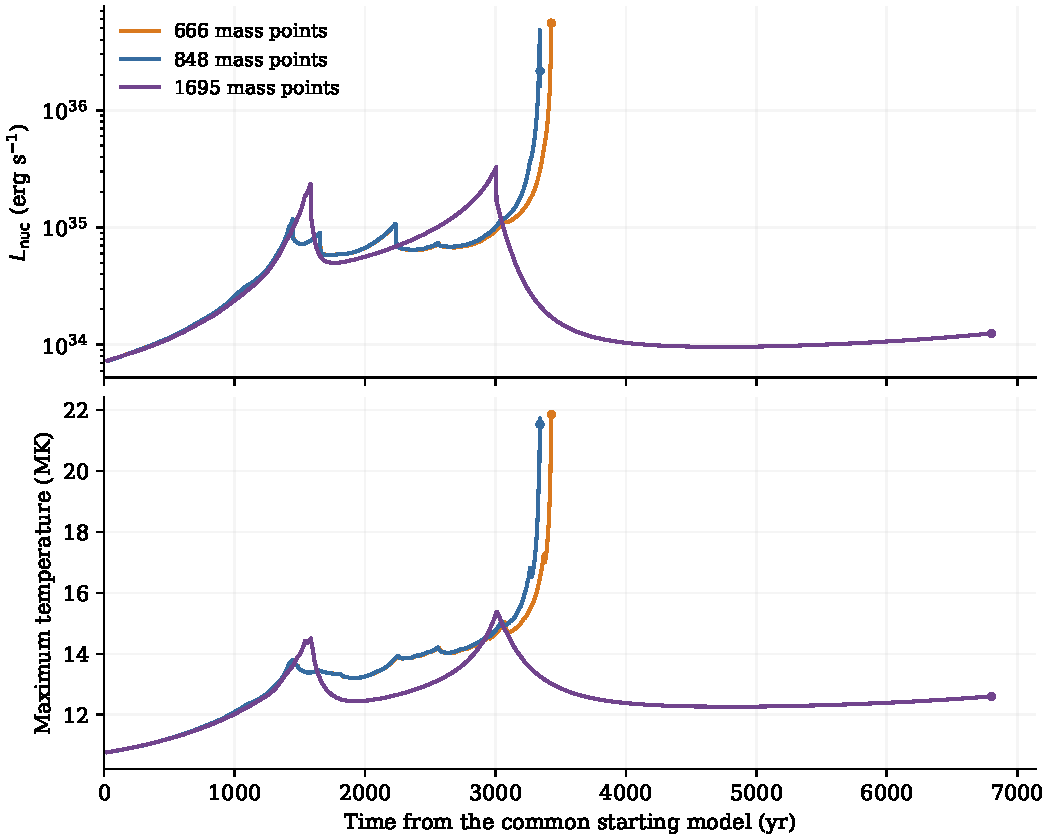
\includegraphics[width=0.92\textwidth]{pulse_face_comparison.pdf}
\caption{Nuclear luminosity and maximum internal temperature on three mass
grids, with total energy and composition enthalpy transported across the
same mass surfaces. All use the white-dwarf table boundary and finite
convective mixing without semiconvection; time runs from the common profile
before shell convection. The largest sampled shell temperatures are
21.86, 21.73 and 15.39 MK; the finest grid reaches 12.60 MK
after a long decline and modest reheating. Sharp decreases near 3006 and
3341 yr are convective-region mergers. Their largest sampled nuclear powers
differ by more than an order of magnitude; the peak is not converged.}
\label{fig:grids}
\end{figure}

\emph{Dependence on the boundary prescription.} Both flash continuations
inherit the white-dwarf table's normalization, which differs from the
TLUSTY boundary by 2.6--3.0\% in temperature and 49--91\% in pressure at the
states sampled. Applying the calculated mixed-to-hydrogen composition ratios
to the hydrogen table retains that normalization rather than testing it.
Comparisons of two extrapolations of the table below $\log g=5.5$, over
$10^3$--$2\times10^6$ yr, change the endpoint temperature by at most
11.27 K and the deposited nuclear energy by at most 0.03\%; these test the
extension, not the absolute boundary. The pulse develops 0.7546 Gyr after
the switch, but that delay does not show that it is independent of the
switch: the shell was fading before it, and the LBA97 model, the grey MESA
sequences and Ember's own grey-boundary sequence (Section~\ref{sec:mesa})
show no flash. Whether ignition survives the original atmosphere can be
decided only by a comparison that starts before the histories diverge. A
pure-hydrogen TLUSTY source rectangle at optical depth 100 above
$\log g=5.95$ is being computed for that control; the 4800 K, $\log g=6.0$
columns are already validated, and the control is pending.

\emph{Mixing physics.} The flash calculations set semiconvective and
thermohaline coefficients to zero. The reaction that powers the flash lowers
the mean molecular weight and can drive thermohaline mixing, as in red
giants \cite{charbonnel07}; whether it does so strongly enough to alter the
shell requires the composition gradient and transport times to be assessed.
Holding the mixing coefficient at its beginning-of-step value during each
implicit solve, as MESA does \cite{paxton11}, passes the species and energy
checks with successive changes of 0.09470\%, 0.04722\% and 0.02357\% in
integrated nuclear energy, but pointwise composition differences do not
decrease.

\subsection{The two continuations}
Two histories were carried through the pulse from the same post-switch
model (Figure~\ref{fig:histories}, Table~\ref{tab:histories}). F1 applies
finite composition transport throughout all convective layers from the onset
of shell convection. F2 first mixes the cooler convective layers
instantaneously, then uses finite transport once the shell convection
connects to the surface envelope; its accumulated thermal and composition
history therefore differs from F1's, and local checks of its later evolution
do not establish that it is F1's outcome. In F2 the envelope becomes
helium-enriched when the convective regions connect: over a checked 0.6656 yr
the surface hydrogen falls from 0.9984 to 0.8085 while helium-3 rises to
0.007264, yet 99\% of the metals remain inside $m/M=0.4456$, so the
atmosphere can be helium-rich while remaining nearly metal-free. Both
histories pass a radius maximum before their temperature maximum: expansion
is followed by contraction during which the surface heats while the
luminosity falls, consistent with delayed structural adjustment. At their
endpoints both are declining in temperature but remain 33--56\%
nuclear-powered, with most of the remaining helium-3 outside the burning
layer. In F2 at $1.345\times10^4$ yr the outer convective envelope, then
4.033\% of the mass, holds 86.44\% of the remaining helium-3 but supplies
0.7504\% of the nuclear power; between $1.443\times10^4$ and
$1.701\times10^4$ yr it loses only 0.01453\% of its helium-3 while the
active layers deplete. The fuel that could power a later episode is
therefore separated from the burning region, and its consumption depends on
transport that these calculations do not yet resolve; fuel depletion alone
does not exclude another unstable episode, and neither history is a
white-dwarf cooling sequence.

\begin{table}[H]\centering\small
\caption{Endpoints of the two flash continuations. Times from the common
model before shell convection; both provisional.}\label{tab:histories}
\begin{tabular}{@{}lrr@{}}\toprule
 & F1 (1983 points) & F2 (2115 points) \\\midrule
Time computed & 5.744 Myr & 42.48 Myr \\
Saved $\Teff$ maximum & 6422 K at 1.139 Myr & 6399 K at 1.088 Myr \\
Endpoint $\Teff$ & 5903 K & 4771 K \\
Endpoint nuclear power (erg s$^{-1}$) & $1.126\times10^{31}$ & $3.166\times10^{30}$ \\
Nuclear share of surface luminosity & 32.84\% & 55.85\% \\
Endpoint radius & $0.09048\Rs$ & $0.05633\Rs$ \\
Surface $X$, $X_3$ & --- & 0.8200, 0.007167 \\
Remaining hydrogen & --- & $0.003792\Ms$ \\
Central $T$, $\rho$ & --- & 6.192 MK, $3.932\times10^4$ g cm$^{-3}$ \\\bottomrule
\end{tabular}
\end{table}

\begin{figure}[H]\centering
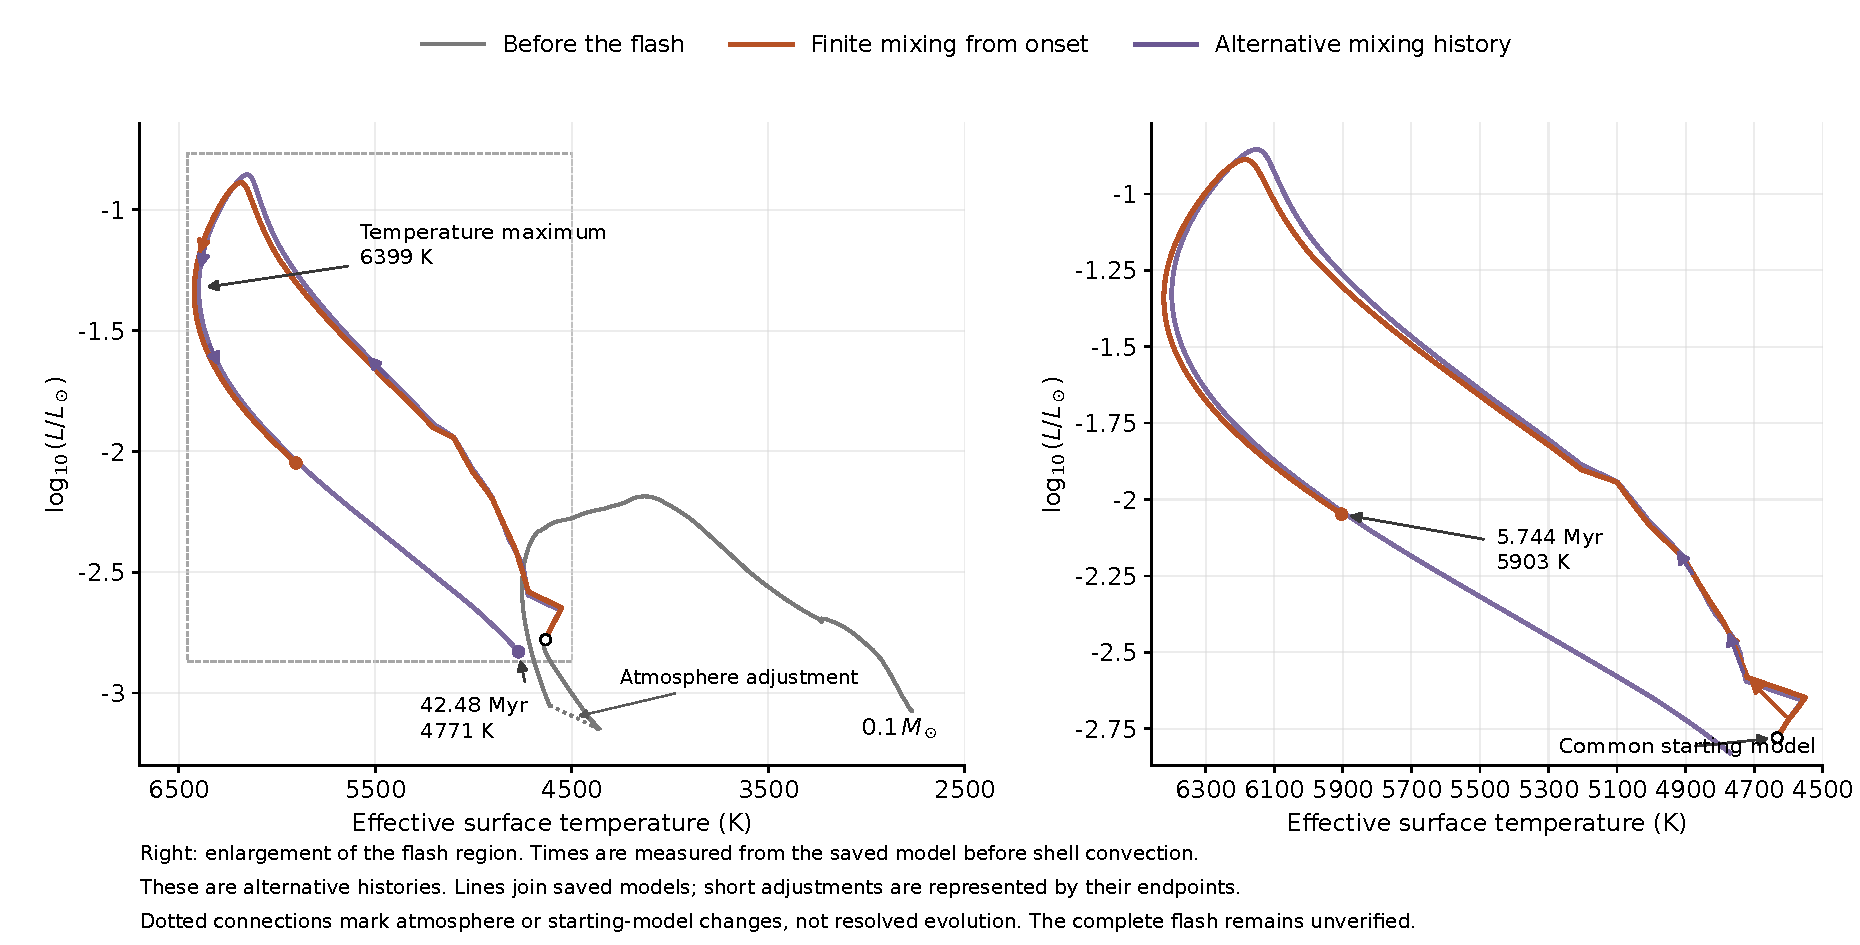
\includegraphics[width=0.95\textwidth]{flash_histories_hr.pdf}\\[4pt]
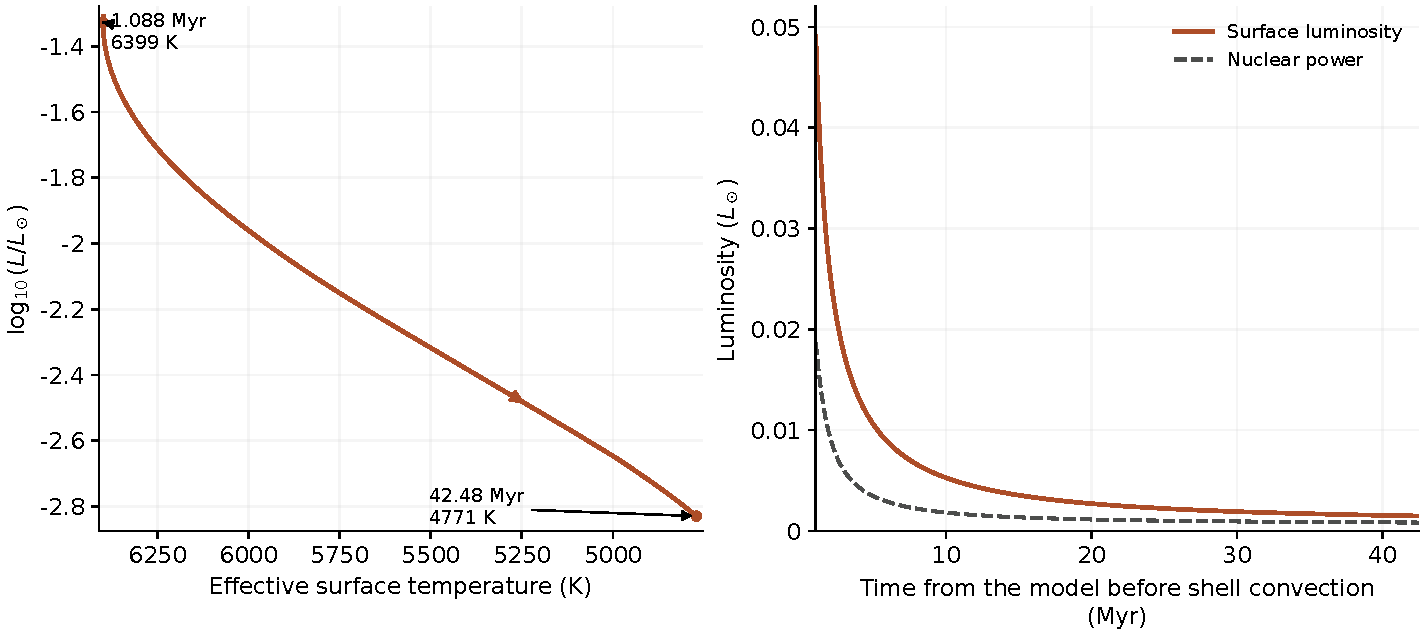
\includegraphics[width=0.95\textwidth]{late_cooling.pdf}
\caption{The two flash continuations. Upper: HR tracks of F1 (orange,
finite mixing from onset) and F2 (purple, alternative mixing history), with
the preceding Track S evolution in gray; dotted connections mark the
atmosphere switch and starting-model adjustments, not resolved evolution.
The right panel enlarges the flash region. Lower: F2 on 2115 points, an
enlarged HR diagram around its temperature maximum (left) and photon
luminosity with deposited nuclear power against time (right). Both
histories use the white-dwarf table boundary switched in at $4.002\Tyr$;
whether the flash occurs with the original atmosphere has not been tested.
Agreement of the two HR tracks does not establish convergence of the peak
power or of the internal mixing.}
\label{fig:histories}
\end{figure}

At 29.48 Myr in F2 the reduced pp network produces helium-3 at
$1.263\times10^{12}$ g s$^{-1}$ and destroys it at $4.106\times10^{11}$
g s$^{-1}$, and helium-3 fusion supplies 23.12\% of the nuclear power,
down from 26.97\% five million years earlier; summing the saved sources
reproduces the inventory change to better than $10^{-10}$. This
establishes the production--destruction balance, not stability against a
later flash. In F2 at 12.07 Myr, 46.16\% of the nuclear power comes from
$^3$He+$^3$He, 49.94\% from the hydrogen reactions that build $^3$He and
3.901\% from the reduced ppII branch; the helium-3 inventory is 82.97\% of
its value in the common starting model. Between $2.012\times10^5$ and
$2.512\times10^5$ yr, nuclear burning supplies 31.97\% of the integrated
surface emission and structural adjustment 68.03\%. The atmosphere tables
entered by the continuations (hydrogen--helium mixtures at 4500--6500 K and
$\log g=4.2$--5.8) were checked for depth and interpolation to better than
0.2\% in temperature and 1.1\% in pressure (Appendix~\ref{app:tech}); the
absolute hydrogen normalization remains the unresolved uncertainty.

\section{Comparisons}\label{sec:comparisons}

\subsection{The published LBA97 model}
LBA97 \cite{lba97} followed the full hydrogen-burning evolution of a
$0.1\Ms$ star into white-dwarf cooling with a grey atmosphere, approximate
opacity changes as hydrogen is consumed, and the interior opacities and
reaction rates of the time. Table~\ref{tab:lba} compares their stated
values with Track P, which is the closest in physics. The starting states
are defined differently: LBA97 includes contraction and defines arrival on
the main sequence by nuclear reactions supplying the whole luminosity, after
about 2 Gyr, whereas Track P starts from a static hydrogen-burning model at
age zero. That offset is small compared with the later differences.

\begin{table}[H]\centering\small
\caption{LBA97 (literature values; curve readings marked $\simeq$) and Track P.}\label{tab:lba}
\begin{tabular}{@{}lrr@{}}\toprule
Quantity & LBA97 & Track P \\\midrule
Initial surface temperature (K) & 2228 & 2766 \\
Initial luminosity ($\Ls$) & $\simeq0.000417$ & 0.0008362 \\
Initial central density (g cm$^{-3}$) & 309 & 381.7 \\
Maximum $^3$He mass fraction & 0.0995 & 0.1003 \\
Age at maximum $^3$He (Tyr) & 1.38 & 0.7103 \\
Radiative layer first forms (Tyr; central $X$) & 5.742 ($\simeq0.16$) & 3.546 (0.1751) \\
Age at hydrogen fraction 0.2034 (Tyr) & $\simeq5.6$ & 3.40 \\
Highest surface temperature (K) & 5807 & $\geq5546$ (endpoint, still rising) \\\bottomrule
\end{tabular}
\end{table}

Ember initially radiates 2.006 times the published luminosity, and the ages
at maximum $^3$He differ by the ratio 1.943. That is what the nuclear clock
requires: with $0.07\Ms$ of hydrogen and about $6\times10^{18}$ erg g$^{-1}$
deposited, the energy supply is of order $8\times10^{50}$ erg and the
burning time is that supply divided by the mean nuclear luminosity, so a
persistently lower luminosity lengthens the clock. A homology estimate gives
the same scale. With $\rho_c\propto R^{-3}$, $T_c\propto R^{-1}$,
$\epsilon_{pp}\propto\rho T^\nu$ for $\nu\simeq4$--6, and nuclear power
equated to $4\pi R^2\sigma\Teff^4$,
\[
R\propto\Teff^{-4/(\nu+5)},\qquad
L\propto\Teff^{4(\nu+3)/(\nu+5)}\simeq\Teff^{3.1\text{--}3.3},
\]
and the temperature ratio predicts a luminosity ratio of 1.959--2.029. The
thermal times $GM^2/(RL)$ are only 3.0 and 5.5 Gyr, so a starting thermal
imbalance cannot sustain a trillion-year offset; the difference lies in the
equilibrium sequence that the physics maintains. The ratios change later in
the evolution, and no single rescaling of time aligns the two calculations.

The low LBA97 luminosity was recognized in 1997: their Section~3.1 reports a
poorer fit to the observed mass--luminosity relation than the Burrows
models. The independent solar-metallicity model of Chabrier and Baraffe
\cite{chabrier97} at $0.1\Ms$ and 1 Gyr gives 2811 K, $0.1240\Rs$ and
$0.0008511\Ls$, close to Ember; they also find that a grey Eddington
boundary generally makes low-mass models hotter, so the grey atmosphere
alone does not explain LBA97's cooler surface. Identifying the cause needs
controlled substitutions of atmosphere, opacity and equation of state, which
have not been done. A reconstruction of the original Fortran program is
available for such tests but does not reproduce LBA97: with two
low-temperature opacity choices it flags a nonconvective centre at 3.307 and
$2.946\Tyr$ (against the published 5.742), and switching only that opacity
changes its luminosity by 54.5\%. Its one close agreement, a highest surface
temperature of 5936 K against 5807 K, does not validate the rest.
Recovering Track P's photospheric density and temperature at optical depth
$2/3$ and plotting them over an opacity map, as in LBA97's Figure~6, shows
the expected drift to hotter, thinner photospheres and nothing that changes
the comparison.

The $^3$He maximum agrees to about 1\%, but Ember reaches it in half the
time and consumes hydrogen faster throughout (Figure~\ref{fig:composition}).
The HR track alone conceals this because it does not show how long the star
spends at each position. Candidate causes are the frequency-dependent
atmospheres, composition-specific opacities, the equation of state and the
updated pp rates; one-ingredient-at-a-time comparisons are needed to
separate them. Agreement with LBA97 is not a measure of accuracy.

\subsection{Independent calculations with MESA}\label{sec:mesa}
We evolved the same mass and bulk composition with the unmodified MESA
release 26.4.1 \cite{jermyn23} in two configurations. Neither shares
Ember's equation of state, opacities, network or atmosphere, so they test
whether an independent code produces the same sequence of events, not the
accuracy of any one ingredient.

\paragraph{Grey-atmosphere configuration.}
MESA starts from pre-main-sequence contraction with its supplied pp/CNO
network, OPAL and low-temperature opacities, electron conduction, an
Eddington grey atmosphere and mixing length 2. Nuclear burning reaches 99\%
of the surface luminosity at 951.3 Myr (3076 K). From that model the
evolution was continued with and without microscopic diffusion. Without
diffusion, central hydrogen crosses 0.001 at $2.372\Tyr$, the surface
reaches its maximum temperature of 6766 K at $2.406\Tyr$, and the model
cools to 595.9 K by $2.564\Tyr$, where the atmosphere requests temperatures
below the 501.2 K floor of the Ferguson opacity table. The final state has
$R=0.02572\Rs$, $L=7.516\times10^{-8}\Ls$, surface $X=0.08778$ and
$0.0009172\Ms$ of hydrogen. This is a computed cooling branch under a grey
boundary; it says nothing about that boundary's accuracy for a cold
helium-rich atmosphere. With diffusion, the same configuration reaches only
$1.225\Tyr$ (3471 K, central $X=0.4593$) in 29.91 CPU-hours: the
atmospheric equation-of-state inversion fails repeatedly on unphysical trial
pressures, a numerical fault rather than a gap along the accepted structure.

\begin{figure}[H]\centering
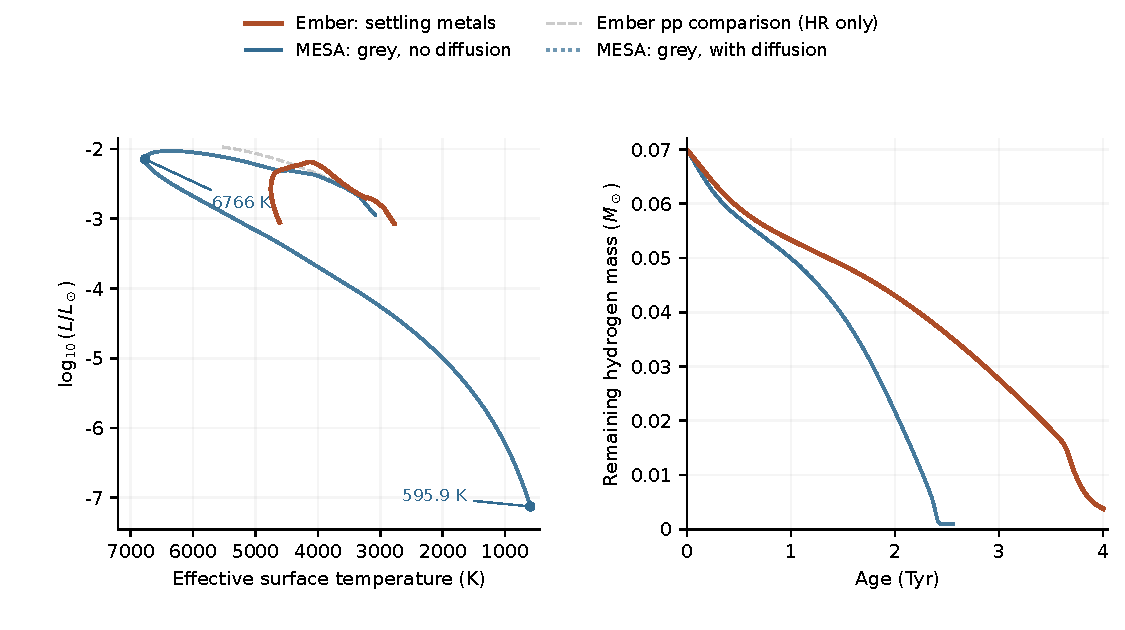
\includegraphics[width=0.85\textwidth]{mesa_comparison.pdf}\\[3pt]
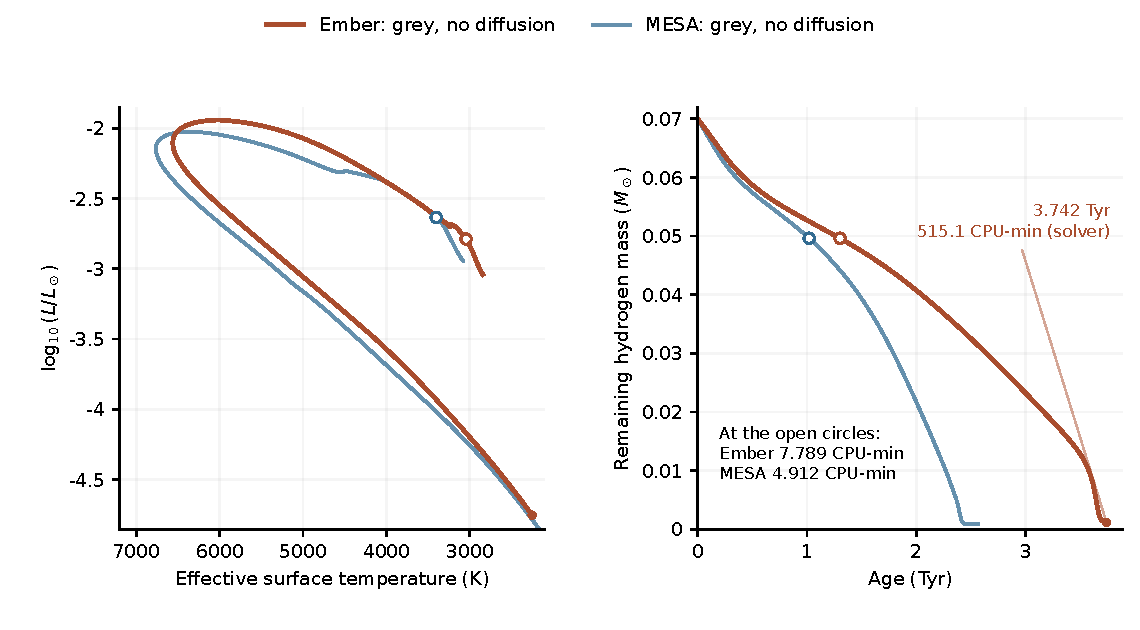
\includegraphics[width=0.85\textwidth]{grey_mesa_comparison.pdf}
\caption{Ember and MESA at $0.1\Ms$. Upper left: HR tracks, including the
computed grey MESA cooling branch; upper right: remaining hydrogen mass.
Solid blue is MESA without diffusion, dotted blue the same grey
configuration with diffusion through $1.225\Tyr$; orange is Track S and
faint dashed gray Track P. Lower: the grey-boundary comparison without
diffusion, Ember (orange, through $3.742\Tyr$) against MESA (blue); open
circles mark equal remaining hydrogen, $0.04963\Ms$, and the filled point
the last Ember model. MESA ages include contraction; Ember ages start at
the static hydrogen-burning model. Equations of state, opacities and
networks differ throughout.}
\label{fig:mesa}
\end{figure}

\paragraph{Ember with the same grey boundary.}
For a like-for-like comparison, an Ember run uses the same Eddington grey
boundary and no microscopic diffusion, with convection, pp+CN burning and
Ember's own equation of state and opacities (Figure~\ref{fig:mesa}). It
reaches $3.742\Tyr$ at 2252 K and central $X=7.991\times10^{-7}$, with a
conductive core at 1.971 MK under a convective envelope. Both codes show the
same transition when a radiative layer separates the core from the envelope:
a luminosity dip and a decline in central helium-3 once replenishment from
the envelope stops. Ember passes it at 3241 K and $3.305\Tyr$ with central
$X=0.1728$; MESA at 4498 K and $2.295\Tyr$ with $X=0.08286$. The difference
in transition temperature and composition is unexplained; the material
physics and time resolution differ, and the transients have not been
compared at matched accuracy. Below 3471 K the Ember grey run includes the
quantum correction to nuclear screening of Potekhin and Chabrier
\cite{potekhin12,chugunov09}, which changes a matched 100 Myr by 0.08920 K.
Neither this sequence nor either MESA sequence develops a helium-3 flash.

At equal remaining hydrogen ($0.04963\Ms$) Ember is at $1.302\Tyr$,
3045 K and $0.001626\Ls$, and MESA at $1.019\Tyr$, 3403 K and
$0.002316\Ls$. Their helium-3 inventories differ ($0.005740$ and
$0.003710\Ms$), so equal hydrogen does not mean equal energy released. To
that point Ember used 7.789 solver CPU-minutes and MESA 4.912 process
CPU-minutes, a ratio of 1.586; the counters have different scope, and a
fully convective phase does not measure relative cost during shell burning
or cooling. Ember's grey sequence used 515.1 solver CPU-minutes through
$3.742\Tyr$ and MESA's grey cooling sequence 1.727 CPU-hours through
750.6 K; these are different phases of different calculations and their
ratio is not a benchmark.

\paragraph{Tabulated-atmosphere configuration.}
The fuller MESA configuration uses PHOENIX and Castelli--Kurucz atmosphere
tables, OPLIB and Ferguson opacities, the blend of FreeEOS, OPAL--SCVH, HELM and Skye equations of state, conduction with the Blouin hydrogen/helium correction, 34 species with
individual diffusion, Ledoux convection with mixing length 1.9 and
Brown--Garaud--Stellmach thermohaline mixing. It has reached only 362 Myr
of contraction (2986 K). Diagnostic runs trace the slowness to diffusion
acting on the thin radiative skin above the convective envelope: when the
diffusion domain becomes active it homogenizes the skin and moves the
atmospheric boundary abruptly. Deepening the diffusion boundary to $10^5$ K
and adding a small mixing coefficient in the outer $10^{-6}$ of the mass
lets a diagnostic run continue to $2.986\Tyr$ (4694 K, central
$X=7.123\times10^{-6}$, surface $X=0.9903$) without retries. These runs
identify a numerical cause; they do not supply a physical surface-mixing
prescription and are not plotted.

A further diagnostic switched a hydrogen-rich MESA model at $3.163\Tyr$
(4737 K, $\log g=6.010$) from the grey boundary to the supplied white-dwarf
table. Within 1000 yr the photon luminosity fell by 19.96\% and the
effective temperature by 5.410\%; over the following 33.65 Myr the model
reached 4176 K with a 15.33\% larger radius. Below $\log g=6$ the MESA
wrapper blends the table with a grey boundary (22.81\% grey weight at the
endpoint), so this is not a pure table continuation. It is the same kind of
boundary change that precedes Ember's flash, and it shows that the response
is an evolving thermal adjustment rather than an equilibrium offset.

\paragraph{What the comparison establishes.}
An independent code with different physics produces the same sequence: full
convection, a radiative layer with a luminosity dip, central hydrogen
exhaustion, a temperature maximum and a turn toward cooling. The ages differ
by about a third between the codes, in the same direction as the LBA97
difference but smaller; given how strongly the nuclear clock depends on
luminosity this is expected rather than diagnostic. The 50 Gyr diffusion
comparison of Section~\ref{sec:hydrogen} shows that element redistribution,
not the omitted oxygen branches, is the stronger candidate for the late
separation between the Ember tracks, although a unique division has not been
measured. Finally, the complete pp/CNO network in MESA does not by itself
make the calculation expensive.

\section{What the model still lacks, and what it would change}\label{sec:limits}
The following omissions are the ones that can change an interpretation in
this paper. For each, the measured size of the effect is given where one
exists.

\paragraph{Atmospheres below 4600 K, above $\log g=6.1$, and without hydrogen.}
Track S stops where its TLUSTY families stop, and the flash continuations
rely on a hydrogen table whose normalization differs from TLUSTY by 49\% in
joining pressure (Section~\ref{sec:flash}). Cooling through 1000, 500 and
100 K requires dense, cool atmospheres with nonideal chemistry,
pressure-dependent and collision-induced absorption, and refraction
\cite{blouin18}. A hydrogen-free atmosphere is not yet possible: the source
programs normalize abundances to hydrogen, and a test at 4017 K shows that
rescaling all number abundances by one factor preserves composition but can
change individual absorption coefficients by a factor of 27.3. These gaps
decide whether a computed cooling age exists at all; nothing in
Sections~\ref{sec:hydrogen}--\ref{sec:flash} is a cooling age.

\paragraph{Grains.}
Equilibrium chemistry finds no condensates in the 3000--3200 K atmospheres
tested nor in the hydrogen-poor structures through 6400 K, but finds them in
the cool upper layers of 2600--2800 K models; dusty models become relevant
near 2800 K and below \cite{chabrier00}. Removing the condensed species from
the gas at 2800 K changes the joining pressure by 0.1246\% and temperature by
$-0.02347\%$. A grain-opacity calculation on one fixed 2800 K profile, with
a condensed mass fraction of $1.094\times10^{-4}$ in $0.1\,\mu$m compact
grains, gives integrated optical depths near $1\,\mu$m of 0.002610
(absorption) and 0.002829 (scattering); coupling grains to the atmospheric
structure and thermodynamics has not been done. Grains are a possible
correction during contraction, the cool initial main sequence and the
eventual cold-remnant phase. The continuous model reaches the main sequence
near 2765 K, so the grain-free assumption also needs assessment there.

\paragraph{Carbon conversion and molecular opacity.}
A fixed metal mixture misrepresents the cool opacity once carbon has been
converted to nitrogen, because CO formation couples the available carbon and
oxygen \cite{lederer09}. Complete conversion of the GS98 carbon captures a
hydrogen mass fraction of $5.728\times10^{-4}$. At $X=0.20$ and
$\rho=5.995\times10^{-6}$ g cm$^{-3}$ the Rosseland absorption mean changes
by the ratios in Table~\ref{tab:cn}; across densities of
$10^{-8}$--$10^{-4}$ g cm$^{-3}$, half conversion raises the 2705 K mean by
18.67--30.22\%. In a coupled 3200 K atmosphere at $\log g=5.15$, half
conversion raises the joining temperature by 1.601\% and lowers the pressure
by 5.681\%; applied to the $3.400\Tyr$ structure for 10 Myr this changes
the luminosity by $-5.162\%$ and the effective temperature by $-1.361\%$. At
5400 K the response is negligible. The effect is material for the cool
part of the track and must be included in a track that carries converted
catalysts to the surface.

\begin{table}[H]\centering\small
\caption{Rosseland absorption mean relative to the fixed GS98 mixture at
$X=0.20$ and $\rho=5.995\times10^{-6}$ g cm$^{-3}$ (gas only).}\label{tab:cn}
\begin{tabular}{@{}rrr@{}}\toprule
$T$ (K) & Half the carbon converted & All the carbon converted \\\midrule
2705 & 1.225 & 1.407 \\
3521 & 1.151 & 1.263 \\
4583 & 0.9971 & 0.9912 \\
5964 & 0.9901 & 0.9744 \\\bottomrule
\end{tabular}
\end{table}

\paragraph{Microscopic transport in degenerate and partially ionized matter.}
At the centre of the $3.890\Tyr$ Track P model the temperature is 0.1506
of the electron Fermi temperature, so degeneracy enters the transport
coefficients, and the thermal-diffusion and heat-flow coefficients must use
one consistent definition \cite{beznogov16,paxton18}. A coupled ion/electron
calculation on the saved gradients, including electron--electron collisions
and the leading ion recoil term, gives provisional outward hydrogen
velocities of $(1.101$--$1.303)\times10^{-9}$ cm s$^{-1}$ at enclosed mass
0.6972, with local drift times $H_P/|w_{\rm H}|$ of 12.78--15.13 Gyr there
and 3.694--4.244 Gyr near mass fraction 0.9738; the thermal force
contributes 23.63--24.48\% of the drift. The range spans two screening
choices and is not an uncertainty. Including electron--electron collisions
gives 0.5277--0.8780 of the elastic-only conductivity across the hot
nonconvective region. These are the coefficients Tracks S and F use above
about 2 MK; below that the tracks represent species exchange by convection
alone, and cold radiative layers still lack a supported transport law.
Heat carried by species motion is at most 0.09557\% of the local luminosity
on hot nonconvective faces; its omission below 2 MK changes surface
luminosity by at most 0.01320\% over 5 Myr.

\paragraph{Interior opacity sources.}
The hot interior opacity comes from one archive, and independent archives
disagree at the few-percent level. On 1940 states with $X=0$ or 0.05 and
$Z=0.01$ or 0.03, the Los Alamos OPLIB means distributed with MESA
\cite{farag24} differ from the TOPS means used here by a median of 2.364\%
and by up to 7.279\%; on 15 warm-envelope layers the Opacity Project
\cite{seaton05} differs from OPLIB by $-9.730$ to $+4.619\%$, and from TOPS
by 2.165\% at a sampled state. The archives use different element sets and
atomic physics, and no track has been run with the alternatives. Where the
sampled layers are convective or conductive the stellar response to opacity
changes of this size is unresolved (Table~\ref{tab:sensitivity}); in the
radiative envelope of the depleted star a $\pm10\%$ change moves the
effective temperature by 3.216 K, so a few-percent archive difference is
below the other uncertainties but is not zero.

\paragraph{The cold helium interior.}
The energy equation used throughout is
$L_\gamma=L_{\rm nuc,dep}+L_{\rm grav}-L_{\nu,\rm thermal}$ with nuclear
neutrinos removed from $L_{\rm nuc,dep}$; at $3.890\Tyr$ in Track P the
terms are 0.01077, $3.201\times10^{-5}$ and (nuclear neutrinos)
$3.362\times10^{-4}\Ls$, with plasma losses of $1.260\times10^{-7}\Ls$ and
a discrete residual below $8\times10^{-11}$. Beyond the computed tracks the
remnant needs a consistent liquid and solid helium free energy with quantum
and mixture effects \cite{baiko22}: specifying melting at $\Gamma=175$ does
not fix the latent heat or the liquid heat capacity. The cold-electron
thermal response, electron and ionic entropies and liquid/solid free
energies have been implemented and checked against thermodynamic identities
and against Ioffe EOSFI22 (largest density-response discrepancy
$1.05\times10^{-6}$ in ideal-ion pressure units), but they are not yet
combined into the production equation of state. Crystallization and its
latent heat, the depth at which convection couples to the isothermal core,
and pycnuclear rates in the actual helium-rich composition \cite{gasques05}
all remain to be evaluated.

\paragraph{Omitted reactions, neutrinos and mixing.}
Pep, hep, ppIII and the oxygen branches are absent in every track; adding a
closed CN cycle to a Track P state adds 2.381\% to the deposited pp energy
and lowers the surface luminosity by 0.1239\% after 5 Myr. Only plasma
neutrino losses are included. Semiconvective heat flux, thermohaline mixing
during the flash, rotation, magnetism, mass loss and accretion are absent.
The tracks describe an isolated, nonrotating star; accretion in particular
would change the surface composition on which the atmosphere depends
\cite{bauer19}.

\paragraph{External heating and encounters.}
Encounters, accretion and particle decay are treated in
Section~\ref{sec:lifetime} as conditional extensions of the isolated track
\cite{adams97}. For close encounters, energy transferred into stellar
oscillations is distinct from retained heat; gravitational radiation can
remove mode energy \cite{rathore05}, and the thermalized fraction must be
determined before it enters a heating history.

\section{Lifetime timeline}\label{sec:lifetime}
The timeline runs from formation to the conditional disappearance of the
remnant. Computed entries are labelled by track and clock; the rest are
literature values or conditional stages whose ages remain to be calculated.
Several late processes can overlap, and disappearance means loss of the
baryonic remnant through decay products.

{\small\renewcommand{\arraystretch}{1.12}
\begin{longtable}{@{}>{\raggedright\arraybackslash}p{0.17\textwidth}>{\raggedright\arraybackslash}p{0.22\textwidth}>{\raggedright\arraybackslash}p{0.56\textwidth}@{}}
\toprule Age or condition & Event & Basis \\\midrule\endfirsthead
\toprule Age or condition & Event & Basis \\\midrule\endhead
Before $t=0$ & Formation and accretion & Cloud collapse, disk and outflows set the mass, entropy and angular momentum; outside the fixed-mass calculation. Low-mass pre-main-sequence models provide the comparison \cite{baraffe15}. \\[3pt]
Contraction clock, 0--1 Gyr & Deuterium burning and contraction & Computed: \pmsTemperature\ K and $\pmsRadius\Rs$ near 1 Gyr with \pmsNuclearPercent\% nuclear support; continued to $\continuousAge\Tyr$ (Section~\ref{sec:contraction}). Lithium depletion is not followed. \\[3pt]
Long-term clock, $t=0$ & Static hydrogen-burning model & Tracks S, F and P start here with $X=0.7$, $\Teff=2766$ K. \\[3pt]
$0.7103\Tyr$ (P) & Maximum $^3$He & Central mass fraction 0.1003, then destruction overtakes production. LBA97: 0.0995 at $1.38\Tyr$. \\[3pt]
$3.546$--$3.551\Tyr$ (P, F, S) & Loss of full convection & A radiative layer separates centre and envelope at central $X\simeq0.175$; the centre becomes radiative near $3.551\Tyr$ in F and S. LBA97: $5.742\Tyr$, $X\simeq0.16$. \\[3pt]
$3.650$--$3.767\Tyr$ (S) & Central hydrogen depletion & Central $X$ crosses $10^{-3}$, $10^{-4}$ and $10^{-5}$; $0.0147\Ms$ of hydrogen remains at the first crossing and burns outside the centre. \\[3pt]
$3.673$, $3.838\Tyr$ (S) & Luminosity and temperature maxima & $0.006513\Ls$; 4754 K. Burning still dominates; no cooling sequence is established. \\[3pt]
$4.002\Tyr$ (S) & Last computed model & 4612 K, central $X=3.528\times10^{-8}$, 97.28\% nuclear. \\[3pt]
Provisional & Helium-3 shell flash & Occurs after a boundary switch; dependence on the original atmosphere untested (Section~\ref{sec:flash}). \\[3pt]
To be calculated & Residual burning fades & Record nuclear heat below 10\%, 1\% and 0.1\% of the photon luminosity, including any recovery. LBA97 reaches 5807 K at its turn; a comparison value only. \\[3pt]
To be calculated & Diffusion and separation & Hydrogen collects at the surface while heavier species settle; a helium core does not imply a helium atmosphere. \\[3pt]
To be calculated & Molecules, grains, dense atmospheres & Follow molecular and collision-induced absorption, condensation and settling where local conditions permit \cite{chabrier00,blouin18}. \\[3pt]
To be calculated & Crystallization and separation & Helium and mixture phase equilibria, latent heat, solid heat capacity; the front follows density and core temperature, not surface temperature \cite{baiko22}. \\[3pt]
To be calculated & Envelope and core couple & Whether and when the convective envelope reaches the nearly isothermal interior; order relative to crystallization unknown. \\[3pt]
$\Teff=1000$, 500, 100 K & Cold-remnant milestones & Record age, core temperature, radius, composition, solid fraction and power sources; below 100 K continue with a solid, partly neutral description. \\[3pt]
$\gtrsim10^{14}$ yr & Changing environment & Retained and ejected objects in evolving stellar and dark-matter environments; accretion of gas, debris and solid bodies is conditional; no unique encounter rate is assumed. \\[3pt]
Close passages & Tidal heating, capture, collision & Distinguish heat from spin and oscillations; couple an encounter survey to waiting-time distributions and post-pulse cooling. \\[3pt]
Allowed interactions & Dark-matter heating & Compare capture, thermalization, evaporation and annihilation with the photon luminosity; include a no-annihilation case \cite{bell24}. \\[3pt]
Nuclear times competitive & Density-driven fusion & Pycnuclear and impurity reactions against cooling and decay times in the helium-rich composition \cite{gasques05}. \\
\bottomrule
\end{longtable}}

\paragraph{Decay and disappearance (conditional).}
Proton decay has not been detected; the Super-Kamiokande partial-lifetime
limit for $p\rightarrow e^+\pi^0$ is $\tau_p/B>2.4\times10^{34}$ yr
\cite{takenaka20}, and baryogenesis does not require it \cite{fukugita86}.
Virtual black holes supply a possible channel with
$\tau_p\sim10^{45}$ yr \cite{adams01}, distinct from the far slower
collective tunnelling of degenerate matter \cite{adams98}. We therefore
carry finite-lifetime scenarios and a stable-baryon branch rather than one
disappearance date. In order of condition, the stages are: decay heating
exceeds cooling and environmental power, possibly long before much mass is
lost; accumulated decays change the composition and mass; degeneracy is
lost and the mass--radius relation must be recalculated for the actual
composition; decay products and then thermal radiation escape as columns
shrink, so that an optically thin object need not radiate as a blackbody;
the remnant ceases to be bound, which is distinct from the decay of every
former baryon; and finally discrete survival replaces a continuous mass. In
the stable-baryon branch cooling, nuclear and environmental alternatives
continue without a decay-imposed endpoint.

\paragraph{A reference clock for the decay era.}
If every baryon has the same constant, independent mean lifetime $\tau_B$,
with no accretion or stable daughters, and $t_d$ measures time from the
start of the comparison,
\begin{equation}
 \langle M_B(t_d)\rangle=M_{B,0}e^{-t_d/\tau_B},\qquad
 L_{\rm heat}=f_{\rm dep}(t_d)\frac{\langle M_B\rangle c^2}{\tau_B},
\end{equation}
where the deposited fraction $f_{\rm dep}$ may evolve and a physical channel
would also account for daughter masses and binding. Half the mass is lost at
$t_d=0.6931\,\tau_B$, 90\% at $2.303$, 99\% at $4.605$ and 99.99\% at
$9.210\,\tau_B$. For $N_0$ independently decaying baryons,
\begin{equation}
 \Pr(t_{\rm last}\leq t_d)=\left(1-e^{-t_d/\tau_B}\right)^{N_0},\qquad
 \langle t_{\rm last}\rangle=\tau_B H_{N_0},
\end{equation}
with $H_N$ the harmonic number. For $0.1\Ms$, $N_0\simeq1.2\times10^{56}$,
the mean last decay occurs near $129.7\,\tau_B$ with a central 90\% interval
of 128.0--132.1$\,\tau_B$. This dates the last of the original baryons,
dispersed or not, not the survival of a bound star. These are analytic
consequences of the stated assumptions, not an extrapolation of any
computed track; a reference lifetime is not a measured age, and changing it
changes temperature, chemistry and energy escape as well as the time scale.

\section{Computing cost and reproducibility}\label{sec:computing}
The model sequences in Figure~\ref{fig:hr} used 47.49 CPU-hours on an
Apple M4 Max: 36.31 for Track S, 10.98 for Track F and 2.259 for Track P,
with 861 shared states (2.052 CPU-hours) counted once. These totals include
table loading, step-doubling comparisons and adaptive retries within the runs
that supply the plotted curves, and exclude independent controls and
discarded tracks. Track S occupied 15.13 hours of elapsed time excluding
pauses between continuations. Building the atmosphere, opacity and
equation-of-state tables that the tracks interpolate cost about 2.6 times
more, roughly 122 CPU-hours for the documented jobs; a rough conversion at
$2\times10^9$ operations per CPU-second, uncertain by a factor of three,
puts the sequences near $3\times10^{14}$ floating-point operations and the
tables near $10^{15}$. The contraction sequence to 1 Gyr took 8.166 CPU
minutes; the continuous run to $2.102\Tyr$ took 66.16 CPU minutes on four
threads. The flash continuations were computed in segments; a complete
cooling-track runtime has not been measured, and none of these numbers
predicts it.

Implicit transport is required: the explicit stability limit of the initial
diffusion coefficients is 672.7--936.1 yr, while accepted steps late on
Track S have a median length of 59.44 Myr among those longer than 1 Myr.
Reusing exactly matching nuclear evaluations reduced the CPU time of a
matched run through $3.757\Tyr$ from 162.4 to 101.8 minutes with identical
output; the other performance changes recorded during development were each
measured in isolation and are not additive.

The repository at \url{https://github.com/oklo/ember} contains the code,
table-generation instructions, the records of input choices and checks,
this paper and the numerical data behind its figures. The LBA97 comparison
records the selected image coordinates, axis calibration and the checksum of
the original PDF, so its curves can be rebuilt without the image. Full raw
outputs, generated physical tables, saved stellar states and executable
archives remain local; regenerating the bulk tables is required before a
stellar calculation can be run from a fresh checkout. Instructions and input manifests for recreating the figures accompany the
paper in the repository.

\appendix
\section{Technical reference}\label{app:tech}

\subsection*{Opacity and equation-of-state continuations}
Settling raises the core metal fraction above the $Z=0.03$ limit of the
tabulated ATOMIC opacities. Through $Z=0.08$ the radiative opacity is
continued linearly from the $Z=0.02$ and 0.03 sources at fixed temperature,
density and hydrogen abundance,
\begin{equation}
 \kappa(T,\rho,X,Z)=\kappa(T,\rho,X,0.03)
 +\frac{Z-0.03}{0.01}\,[\kappa(T,\rho,X,0.03)-\kappa(T,\rho,X,0.02)],
\end{equation}
with all source temperature and density bounds enforced. Transferring the
OPLIB composition ratio from $Z=0.02$ to a withheld $Z=0.03$ source differs
from the ATOMIC value by at most 0.1867\% at 34 core states, and the linear
and ratio forms differ by 0.001212\% in luminosity over a matched 5 Gyr.
Independent OPLIB data through $Z=0.2$ support linear scaling within
3.302\% at 6--10 MK; in the region with $Z>0.06$ radiation carries at most
0.04154\% of the gradient-driven heat. As the envelope falls below
$Z=0.01$ the molecular opacity interpolates the actual AESOPUS values,
including $Z=0$ and 0.004; at higher temperatures $\kappa$ is continued
linearly in $Z$ from the 0.01 and 0.02 sources with a floor at
$Z=10^{-4}$. Hydrogen dependence is continued in $\log\kappa$ from the
$X=0.70$ and 0.75 sources through pure hydrogen; the molecular source ends
at $1-X=10^{-7}$. In the dense hydrogen envelope, where the OPLIB table
ends at $\log R=1.5$ ($R=\rho/T_6^3$), the TOPS hydrogen slope is blended
in over $\log R=1.25$--1.45 and used to $\log R\leq1.8$ for
$\log T=5.6$--6.1; convection carries 99.96\% of the heat at the affected
layer. In dense core cells without spectral coverage (0.125--0.45 keV,
$10^4$--$10^5$ g cm$^{-3}$, $X\leq0.2$) the tabulated uncut opacity is
multiplied by an inferred plasma correction; radiation carries at most
0.2535\% of the local transport there.

The variable-metal equation-of-state family covers $Z=0$--0.08 (0.16 for
the core) and all 23 sampled Track S structures. Against direct FreeEOS
evaluations the maximum differences are 0.03028\% in pressure, 0.09056\% in
adiabatic gradient, 0.7642\% in heat capacity and 1.037\% in $\Gamma_1$;
36 low-density and 28 high-metal comparisons agree within 0.009197\% and
0.02530\% in the material responses. The Track F family (152 tables, 38
hydrogen and four $^3$He fractions) has a maximum second-composition-derivative
difference of 0.1499\% at 102 compositions and a heat-capacity difference of
0.1062\% on the saved 512-point structure. Composition derivatives are
evaluated without an abundance floor, including when a species is exactly
absent; 128 analytic comparisons and five FreeEOS curvature checks at zero
$^3$He (within 0.007181\%) pass. The continuous driver's potential matches
direct FreeEOS to 0.02589\% in pressure and 0.02467\% in internal energy on
the 512-zone reference profile.

\subsection*{Atmosphere families}
Table~\ref{tab:atm} lists the atmosphere tables entered by Track S and the
flash continuations. ``Depth'' is the largest change in joining temperature
and pressure when the source column is computed to a deeper lower boundary;
``interpolation'' is the largest difference between an independently solved
column and the interpolated value. Missing cells remain inaccessible to the
evolution rather than being filled.

{\small\renewcommand{\arraystretch}{1.1}
\begin{longtable}{@{}>{\raggedright\arraybackslash}p{0.30\textwidth}>{\raggedright\arraybackslash}p{0.22\textwidth}rp{0.12\textwidth}p{0.16\textwidth}@{}}
\caption{Atmosphere tables along Track S and the flash continuations.}\label{tab:atm}\\
\toprule Composition & $\Teff$ (K), $\log g$ & Columns & Depth ($T$; $P$) & Interpolation ($T$; $P$) \\\midrule\endfirsthead
\toprule Composition & $\Teff$ (K), $\log g$ & Columns & Depth ($T$; $P$) & Interpolation ($T$; $P$) \\\midrule\endhead
Track P reference: $X=0.1$--0.7, $X_3=0$--0.12, $Z=0.02$ & to 5600; 4.9--5.4 & 220 & 0.007883\% & 0.7399\%; 0.5707\% \\
Warm extension, $X=0.15$, 0.2 & 5400--6400; 5.7, 6.0 & 300 & 0.009372\% & 0.4860\% \\
Late Track F grid, $X=0.70$--0.90, $X_3=0$--0.03 & 3400--4000; 4.9--5.15 & 48 & --- & 1.837\% in $T$ \\
Metal response $Z=0.01$--0.02 (paired) & to 4400; 5.025 & pairs & 0.0002576\% & 0.6093\%; 3.064\% \\
$Z=0.005$--0.01 & to 4400; 5.1 & pairs & --- & 1.671\%; 1.980\% \\
$Z=0.0025$--0.005 & to 4400; 5.1 & 12 pairs & 0.001301\%; 0.002243\% & 0.03091\%; 0.2311\% \\
$Z=0.001$--0.0025 & 4000--4400; 5.1 & 8 pairs & --- & 0.2539\%; 3.111\% \\
$Z=0.0005$--0.001 & 4000--4400; 5.1 & 8 pairs & --- & 2.031\%; 2.755\% \\
$X=0.9$--0.98, $Z=0.001$, $X_3=0$, 0.003 & 4000--4800; 4.9--5.4 & 70 & --- & 0.004095\%; 0.01689\% \\
$X=0.995$--0.9995, $Z=10^{-6}$--$10^{-4}$ & 4600--5200; 5.15--5.65 & 94 & --- & 0.09719\%; 4.656\% \\
$1-X=10^{-5}$--$10^{-3}$, $Z=10^{-8}$--$10^{-6}$ & 4600--5200; 5.4--5.65 & 81 & (shallowest ends at $\tau=168.3$) & 0.4624\%; 0.3930\% \\
$Z\leq10^{-6}$, He $10^{-10}$ & 4700--6000; 5.5--5.95 & 72 & $4.327\times10^{-6}$\%; $4.770\times10^{-5}$\% & 0.1751\%; 0.5986\% \\
Zero metal, cold & 4650--4800; 5.9--5.95 & 6 & below $10^{-6}$ & 0.1154\%; 1.108\% \\
Gravity continuation & 4650--4800; 5.95--6.1 & inferred & --- & 0.1878\%; 2.391\% (9 solved) \\
Temperature continuation & 4600; 5.9 & 1 solved & --- & within 0.05\% \\
H--He mixtures (flash), $X=0.78$--0.9955 & 4500--5500; 4.95--5.80 & 54 & 0.02452\%; 0.03703\% & 0.08784\%; 1.094\% \\
H--He mixtures, three $X$ & 4700--6000; 4.95--5.25 & 36 & 0.01078\%; 0.06911\% & --- \\
H--He mixtures, three $X$ & 6000--6500; 4.20--5.55 & 60 & 0.01373\%; 0.09599\% & --- \\
H--He mixtures, three $X$ & 5000--6000; 5.4--5.8 & 27 & --- & $7.587\times10^{-6}$\%; 0.1582\% \\
MESA hydrogen white-dwarf table \cite{mesa_atm} & 2000--40,000; 5.5--9.5 & table & joined at $\tau=25.12$ & extrapolated below $\log g=5.5$ \\
\bottomrule
\end{longtable}}

Within $0.90<X<0.94$ the logarithms of the joining values are interpolated
in hydrogen between the $X=0.90$ and 0.94 families; the metal response is
calibrated at $X_3=0$ and applied separately from the small isotope
response, and helium below a mass fraction 0.005 is neglected in the
4600--4800 K, $\log g=5.9$--6.1 domain (solved helium-bearing columns change
the joining values by less than 0.1\% in $T$ and 2.5\% in $P$). In the flash
continuations the hydrogen table is extrapolated below $\log g=5.5$ using
either its lowest two rows or the gravity response of solved near-hydrogen
atmospheres at $\log g=4.35$ and 4.50; the two inferred references differ by
up to 2.189\% in temperature and 15.04\% in pressure at tabulated points,
and paired stellar comparisons between them are those quoted in
Section~\ref{sec:flash}.

\subsection*{Time-step and conservation checks}
Every accepted interval compares one full step with two half steps in
structure, species, total hydrogen and energy. Species balances are checked
independently in each composition region together with the inert-metal
mass, nuclear rest-mass release and the first law. For Tracks S, F and P, the relative time-error
budgets are 0.0003 for radius, density and temperature, 0.003 for local
$^3$He and 0.001 for the other species; the abundance solver tolerance is
$10^{-10}$ with a stricter fallback (a $10^{-12}$ control changes mass
fractions by at most $1.360\times10^{-10}$). During the flash, deposited
nuclear energy is integrated consistently with the implicit equations, time
refinement permits 0.5\% in deposited energy and 0.1\% in structure and
endpoint nuclear power (a 1\% allowance was tested and rejected because a
local temperature difference of $|\Delta\ln T|=0.001091$ exceeded the
declared 0.001 limit), and the first-law residual is measured against the
larger of nuclear and photon luminosity with a limit of $2\times10^{-8}$.
Mesh insertions preserve species inventories, internal energy and the nodal
gravitational-energy sum. Increasing the separate abundance-change limit per
step from 0.001 to 0.005 saves 24.99\% of CPU over a matched 1 Gyr with a
luminosity change of 0.0005727\%; a larger structure tolerance was rejected
(Section~\ref{sec:model}). Electron-pair collision integrals for the late
shell-burning calculation cover degeneracy parameter $\eta=-6$--64 and
screening parameter $b=0.1$--2400, with interpolation and integration checks
within 0.3466\%. Collision integrals use 96 Jacobi and 128 Legendre points;
against 384/512 points the maximum scaled coefficient difference is
$4.851\times10^{-9}$.

\begin{thebibliography}{99}\small
\bibitem{jermyn23} Jermyn, A. S., et al. (2023).
Modules for Experiments in Stellar Astrophysics (MESA): Time-Dependent
Convection, Energy Conservation, Automatic Differentiation, and Infrastructure.
\emph{ApJS}, 265, 15. \url{https://arxiv.org/abs/2208.03651}.
\bibitem{mesa_atm} MESA documentation. Table atmospheres.
\url{https://docs.mesastar.org/en/latest/atm/table.html}.
\bibitem{rohrmann11} Rohrmann, R. D., Althaus, L. G., \& Kepler, S. O. (2011).
Lyman $\alpha$ wing absorption in cool white dwarf stars.
\emph{MNRAS}, 411, 781--791.
\href{https://doi.org/10.1111/j.1365-2966.2010.17716.x}{doi:10.1111/j.1365-2966.2010.17716.x}.
\bibitem{colgan16} Colgan, J., et al. (2016).
A New Generation of Los Alamos Opacity Tables. \textit{ApJ}, 817, 116.
\href{https://doi.org/10.3847/0004-637X/817/2/116}{doi:10.3847/0004-637X/817/2/116}.
\bibitem{tops} Los Alamos National Laboratory. TOPS opacity service,
ATOMIC/New elemental library and mixture queries.
\href{https://aphysics2.lanl.gov/opacity/lanl/}{aphysics2.lanl.gov/opacity/lanl/}.
\bibitem{davis24} Davis, Y. T., et al. (2024).
The EBLM Project XII. An eccentric, long-period eclipsing binary with a companion
near the hydrogen-burning limit.
\href{https://arxiv.org/pdf/2312.09156v2}{arXiv:2312.09156v2}, Table 2 and abstract.
\bibitem{agol21} Agol, E., et al. (2021).
Refining the Transit-timing and Photometric Analysis of TRAPPIST-1:
Masses, Radii, Densities, Dynamics, and Ephemerides.
\href{https://arxiv.org/pdf/2010.01074}{arXiv:2010.01074}, Table 7.
\bibitem{ribas17} Ribas, I., et al. (2017).
The full spectral radiative properties of Proxima Centauri.
\href{https://arxiv.org/pdf/1704.08449}{arXiv:1704.08449}, Table 11.
\bibitem{lba97} Laughlin, G., Bodenheimer, P., \& Adams, F. C. (1997).
The End of the Main Sequence. \emph{ApJ}, 482, 420.
\href{https://doi.org/10.1086/304125}{doi:10.1086/304125}.
\bibitem{chabrier97} Chabrier, G., \& Baraffe, I. (1997).
Structure and evolution of low-mass stars. \emph{A\&A}, 327, 1039.
\href{https://arxiv.org/abs/astro-ph/9704118}{arXiv:astro-ph/9704118}, Table 2.
\bibitem{adams97} Adams, F. C., \& Laughlin, G. (1997).
A dying universe: the long-term fate and evolution of astrophysical objects.
\emph{Rev. Mod. Phys.}, 69, 337.
\href{https://doi.org/10.1103/RevModPhys.69.337}{doi:10.1103/RevModPhys.69.337}.
\bibitem{rathore05} Rathore, Y., Blandford, R. D., \& Broderick, A. E. (2005).
Resonant excitation of white dwarf oscillations in compact object binaries---I.
The no back reaction approximation.
\emph{MNRAS}, 357, 834.
\href{https://academic.oup.com/mnras/article/357/3/834/1077414}{Published calculation}.
\bibitem{hrw94} Haft, M., Raffelt, G., \& Weiss, A. (1994).
Standard and nonstandard plasma neutrino emission revisited.
\href{https://arxiv.org/abs/astro-ph/9309014}{arXiv:astro-ph/9309014}.
\bibitem{chabrier00} Chabrier, G., Baraffe, I., Allard, F., \& Hauschildt, P. (2000).
Evolutionary models for very low-mass stars and brown dwarfs with dusty atmospheres.
\emph{ApJ}, 542, 464.
\href{https://arxiv.org/abs/astro-ph/0005557}{arXiv:astro-ph/0005557}.
\bibitem{baiko22} Baiko, D. A., \& Chugunov, A. I. (2022).
\emph{Ab initio} thermodynamics of one-component plasma for astrophysics of
white dwarfs and neutron stars.
\href{https://arxiv.org/abs/2112.04822}{arXiv:2112.04822}.
\bibitem{blouin18} Blouin, S., Dufour, P., \& Allard, N. F. (2018).
A new generation of cool white dwarf atmosphere models. I. Theoretical framework
and applications to DZ stars.
\href{https://arxiv.org/abs/1807.06616}{arXiv:1807.06616}.
\bibitem{beznogov16} Beznogov, M. V., Potekhin, A. Y., \& Yakovlev, D. G. (2016).
Diffusive heat blanketing envelopes of neutron stars.
\emph{MNRAS}, 459, 1569.
\href{https://doi.org/10.1093/mnras/stw751}{doi:10.1093/mnras/stw751}.
\bibitem{thoul94} Thoul, A. A., Bahcall, J. N., \& Loeb, A. (1994).
Element diffusion in the solar interior. ApJ, 421, 828.
\href{https://arxiv.org/abs/astro-ph/9304005}{arXiv:astro-ph/9304005}.
\bibitem{denissenkov13} Denissenkov, P. A., Herwig, F., Bildsten, L.,
\& Paxton, B. (2013). MESA Models of Classical Nova Outbursts: The Multicycle
Evolution and Effects of Convective Boundary Mixing. \emph{ApJ}, 762, 8.
\href{https://doi.org/10.1088/0004-637X/762/1/8}{Published article}.
\bibitem{bauer19} Bauer, E. B., \& Bildsten, L. (2019).
Polluted White Dwarfs: Mixing Regions and Diffusion Timescales.
\emph{ApJ}, 872, 96. \href{https://arxiv.org/abs/1812.09602}{arXiv:1812.09602}.
\bibitem{charbonnel07} Charbonnel, C., \& Zahn, J.-P. (2007).
Thermohaline mixing: A physical mechanism governing the photospheric
composition of low-mass giants. \emph{A\&A}, 467, L15.
\href{https://arxiv.org/abs/astro-ph/0703302}{arXiv:astro-ph/0703302}.
\bibitem{paxton11} Paxton, B., et al. (2011).
Modules for Experiments in Stellar Astrophysics (MESA).
\emph{ApJS}, 192, 3.
\href{https://doi.org/10.1088/0067-0049/192/1/3}{Published methods}.
\bibitem{paxton18} Paxton, B., et al. (2018).
Modules for Experiments in Stellar Astrophysics (MESA): Convective Boundaries,
Element Diffusion, and Massive Star Explosions.
\href{https://arxiv.org/abs/1710.08424}{arXiv:1710.08424}, section 3.2.2.
\bibitem{adelberger11} Adelberger, E. G., et al. (2011).
Solar fusion cross sections. II. The pp chain and CNO cycles.
Reviews of Modern Physics, 83, 195.
\bibitem{acharya25} Acharya, B., et al. (2025).
Solar fusion III: New data and theory for hydrogen-burning stars.
\emph{Rev. Mod. Phys.}, 97, 035002.
\href{https://doi.org/10.1103/8lm7-gs18}{doi:10.1103/8lm7-gs18}.
\bibitem{baraffe15} Baraffe, I., Homeier, D., Allard, F., \& Chabrier, G. (2015).
New evolutionary models for pre-main sequence and main sequence low-mass stars
down to the hydrogen-burning limit.
\href{https://arxiv.org/abs/1503.04107}{arXiv:1503.04107}.
\bibitem{takenaka20} Takenaka, A., et al. (Super-Kamiokande Collaboration, 2020).
Search for proton decay via $p\to e^+\pi^0$ and $p\to\mu^+\pi^0$
with an enlarged fiducial volume in Super-Kamiokande I--IV.
\href{https://arxiv.org/abs/2010.16098}{arXiv:2010.16098}.
\bibitem{fukugita86} Fukugita, M., \& Yanagida, T. (1986).
Baryogenesis without grand unification. \emph{Phys. Lett. B}, 174, 45.
\href{https://doi.org/10.1016/0370-2693(86)91126-3}{doi:10.1016/0370-2693(86)91126-3}.
\bibitem{adams98} Adams, F. C., Laughlin, G., Mbonye, M., \& Perry, M. J. (1998).
The gravitational demise of cold degenerate stars. \emph{Phys. Rev. D}, 58, 083003.
\href{https://arxiv.org/abs/astro-ph/9808250}{arXiv:astro-ph/9808250}.
\bibitem{adams01} Adams, F. C., Kane, G. L., Mbonye, M., \& Perry, M. J. (2001).
Proton decay, black holes, and large extra dimensions.
\href{https://arxiv.org/abs/hep-ph/0009154}{arXiv:hep-ph/0009154}.
\bibitem{bell24} Bell, N. F., et al. (2024).
Heavy Dark Matter in White Dwarfs: Multiple-Scattering Capture and Thermalization.
\href{https://arxiv.org/abs/2404.16272}{arXiv:2404.16272}.
\bibitem{gasques05} Gasques, L. R., et al. (2005).
Nuclear fusion in dense matter: Reaction rate and carbon burning.
\emph{Phys. Rev. C}, 72, 025806.
\href{https://arxiv.org/abs/astro-ph/0506386}{arXiv:astro-ph/0506386}.
\bibitem{lederer09} Lederer, M. T., \& Aringer, B. (2009).
Low temperature Rosseland opacities with varied abundances of carbon and nitrogen.
\href{https://doi.org/10.1051/0004-6361:200810576}{Published article};
\href{https://arxiv.org/abs/0810.5672}{arXiv:0810.5672}.
\bibitem{potekhin12} Potekhin, A. Y., \& Chabrier, G. (2012).
Thermonuclear fusion in dense stars: Electron screening, conductive cooling,
and magnetic field effects. A\&A, 538, A115.
\href{https://arxiv.org/abs/1201.2133}{arXiv:1201.2133}.
\bibitem{chugunov09} Chugunov, A. I., \& DeWitt, H. E. (2009).
Nuclear fusion reaction rates for strongly coupled ionic mixtures.
Physical Review C, 80, 014611.
\href{https://arxiv.org/abs/0905.3844}{arXiv:0905.3844}.
\bibitem{seaton05} Seaton, M. J. (2005).
OP data on CD for mean opacities and radiative accelerations.
\href{https://doi.org/10.1111/j.1365-2966.2005.00019.x}{doi:10.1111/j.1365-2966.2005.00019.x}.
\bibitem{farag24} Farag, E., et al. (2024).
An Expanded Set of Los Alamos OPLIB Tables in MESA:
Type-1 Rosseland-mean Opacities and Solar Models.
\textit{The Astrophysical Journal}.
\href{https://doi.org/10.3847/1538-4357/ad4355}{doi:10.3847/1538-4357/ad4355}.
\end{thebibliography}

\end{document}
